%%%%%%%%%%%%%%%%%%%%%%%%%%%%%%%%%%%%%%%%%
% Masters Degree Thesis 
% Use pdflatex to compile  
% Note:
% All document variables are stored in the Thesis.cls file
%
%%%%%%%%%%%%%%%%%%%%%%%%%%%%%%%%%%%%%%%%%

%----------------------------------------------------------------------------------------
%	PACKAGES AND OTHER DOCUMENT CONFIGURATIONS
%----------------------------------------------------------------------------------------

\documentclass[11pt, oneside]{Thesis} % The default font size and one-sided printing

\graphicspath{{Pictures/}} % The directory where pictures are stored

\usepackage[square, numbers, url, comma, sort&compress, tocloft, cite]{natbib}
\usepackage[a4paper,lmargin=2.6in,rmargin=0in,tmargin=2.5in,bmargin=0in]{geometry}
\usepackage{sectsty}
\usepackage[center]{titlesec}
\hypersetup{urlcolor=black, colorlinks=true} % Colors hyperlinks in black
\title{\ttitle} % Defines the thesis title
\newcommand*{\justifyheading}{\raggedright}
\newcommand*{\justifyhead}{\centering}
\titleformat{\chapter}[display]
  {\normalfont\huge\bfseries\justifyhead}{\chaptertitlename\ \thechapter}
  {20pt}{\Huge}
\titleformat{\section}
  {\normalfont\Large\bfseries\justifyheading}{\thesection}{1em}{}
\titleformat{\subsection}
  {\normalfont\large\bfseries\justifyheading}{\thesubsection}{1em}{}
\begin{document}

%----------------------------------------------------------------------------------------
%	TITLE PAGE
%----------------------------------------------------------------------------------------
\frontmatter % Use Roman page numbering style (i, ii, iii, iv...) for pre-content pages

\begin{titlepage}
\begin{center}
\textsc{\Large \textbf{UNIVERSITY OF BUEA}}\\[25pt]\\[3.0cm] % University of Buea
\end{center}

\begin{minipage}{0.5\textwidth}
\begin{flushleft}
\large\textbf{FACULTY OF SCIENCE}
\end{flushleft}
\end{minipage}
\begin{minipage}{0.5\textwidth}
\begin{flushright}
\large\textbf{DEPARTMENT OF COMPUTER}\\  
\end{flushright}
\end{minipage}
\large \hspace*{275} \textbf{SCIENCE}
\hspace{200}\\

\begin{center}
\\[1.5cm]
{\large \bfseries IMPLEMENTATION OF A HEART-SHAPED PRIMITIVE}\\[0.4cm] % Implementation of a Heart-Shaped Primitive
\\[2.5cm]

\large \textbf{ By } \\[0.75cm]

\Large \textbf{\authornames} \\ 

\small B.Sc. (Hons) Mathematics \\[2.5cm]

\large \textbf{A Thesis Submitted to the Department of Computer Science, \\
		Faculty of Science, University of Buea, in Partial Fulfilment \\ 
		of the Requirements for the Award of the \\
		Master of Science (M.Sc.) Degree \\
		in Computer Science}\\[2.5cm]

\large \textbf{July, 2015}

\end{center}

\end{titlepage}

%----------------------------------------------------------------------------------------
%	DEDICATION PAGE
%----------------------------------------------------------------------------------------
\Dedication{
\pagestyle{plain} % No headers or footers for the following pages
\begin{center}\Large To My Family \end{center}

\vfill\vfill\vfill\vfill\vfill\vfill\null % Add some space at the bottom to position the quote just right
}
\clearpage % Start a new page

%----------------------------------------------------------------------------------------
%	CERTIFICATION PAGE
%----------------------------------------------------------------------------------------

\begin{center}
\textsc{\Large \textbf{UNIVERSITY OF BUEA}}\\[25pt]\\[0.5cm] % University of Buea
\end{center}

\begin{minipage}{0.5\textwidth}
\begin{flushleft}
\large\textbf{FACULTY OF SCIENCE}
\end{flushleft}
\end{minipage}
\begin{minipage}{0.5\textwidth}
\begin{flushright}
\large\textbf{DEPARTMENT OF COMPUTER}
\end{flushright}
\end{minipage}
\large \hspace*{275} \textbf{SCIENCE}

\Certification{

\addtocontents{toc} % Add a gap in the Contents

The thesis of \authornames\hspace{2}(SC09B676) entitled: “\textbf{\ttitle}” submitted to the \deptname, \facname\hspace{4}at the \univname\hspace{3} in partial fulfillment of the requirements for the award of the Master of Science (M.Sc.) degree in Computer Science has been examined and approved by the examination panel composed of:\\

\hspace*{1em}Ngwa A. Gideon (Ph.D), Chairperson ( Associate Professor of Mathematics )\\
\hspace*{1em}Nkweteyim L. Denis (Ph.D), Examiner ( Lecturer of Computer Science )\\
\hspace*{1em}Kamgnia Emmanuel (Ph.D), Supervisor (Lecturer of Computer Science )\\[0.5cm]

\Large \textbf{-------------------------------}\hspace*{80}\textbf{--------------------------------}
\Large \hspace{95} Nkweteyim L. Denis (PhD) \hspace*{80} Kamgnia Emmanuel (PhD)\\
\large\hspace*{2em} (Head of Department) \hspace*{155} (Supervisor)\\[1.0cm]

\Large This thesis has been accepted by the Faculty of Science.\\[0.5cm]

\Large \textbf{Date:}\textbf{----------------------------}\hspace*{80}\textbf{---------------------------} 
\hspace*{19em}Prof. Ayonghe N. Samuel\\ 
\large \hspace*{28em}( Dean )
}
\clearpage % Start a new page

%----------------------------------------------------------------------------------------
%	ACKNOWLEDGEMENTS
%----------------------------------------------------------------------------------------
\Acknowledgement{

\addtocontents{toc}% Add a gap in the Contents,
\\
Firstly, I thank our Lord Jesus Christ for giving me
life and good health during my stay at University Of Buea and for
granting me the patience to go through this program.

I am grateful to the Vice Chancellor of the University Of Buea and her collaborators for 
maintaining an enabling environment where graduate students can  
learn and express their utmost research potential. I am especially indebted  
to Professor Joyce B.M. Endeley, former Director of the Higher  
Technical Teachers’ Training College of the University of Buea in Kumba  
and Professor Theresa Nkuo­ Akenji, the former Deputy Vice Chancellor for  
Internal Control and Evaluation who authorized the connection of internet  
facilities to the Postgraduate Computer Science Laboratory during the  
implementation of this project.
I wish to sincerely thank all the staff of the Department of Computer  
Science for their advice and stimulating conversations during the writing of  
this thesis. Special thanks go to Dr. Denis Nkweteyim and Professor Emmanuel Kamgnia 
for meticulously proofreading through and correcting this work while 
making their wide spectrum of research experience and books  
on graphics available to me.

My appreciation goes to the Google Open Source Programs
Office (OSPO) – Mary Radomile, Carols Smith, Cat Allman and
Stephanie Taylor, as well as the United States Army Research Laboratory BRL-CAD team
 for their sponsorship of this project under the auspices
of the 2013 Google Summer Of Code program. Special thanks go
to Mr.Christopher Sean Morrison and Mr.Erik Greenwald for their
valuable advice and mentorship during the implementation of this
project. I am also indebted to Juoko Orava aka \textit{Nominal Animal} and the
mathematician Dr.Titus Piezas for tips on ray-tracing the heart
surface.

Many thanks go to my family for their assistance and
encouragement throughout this program.This thesis is dedicated to them.
I also thank the friends I made during the
course of this program whether from University of Buea or the Developer community,
for bringing all the fun they came along with– I appreciate your
company and I'm happy to know I was not alone.
}
\clearpage % Start a new page

%----------------------------------------------------------------------------------------
%	ABSTRACT PAGE
%----------------------------------------------------------------------------------------
\Abstract{

\abstract{\addtocontents{toc}%Add a gap in the Contents

This thesis titled \ttitle \hspace{2} was aimed at demonstrating the engineering of a heart-shaped primitive within the BRL-CAD ( Ballistic Research Laboratory Computer Aided Design ) package. Using a case study approach, the heart-shaped primitive's data structure was designed, necessary callback functions were written and tested with BRL-CAD's testing infrastructure. It was shown that the Laguerre-based root solver is indeed a sure-fire iterative method for finding roots of polynomials and it's stability on sextic equations was ascertained. Also, this work provided a guideline for the development of primitives within open source Computer Aided Design (CAD) software and showed that the BRL-CAD package primarily developed for the military sector can be used in non-military locales for entertainment purposes. \\[0.5cm]
\textbf{Keywords: } \keywordnames
}
}
\clearpage % Start a new page

%----------------------------------------------------------------------------------------
%	TABLE OF CONTENTS
%----------------------------------------------------------------------------------------

\pagestyle{plain} % Use the "plain" headers as defined before to bring them back
\lhead{\emph{Table of Contents}}

\Large \hspace*{125} \textbf{TABLE OF CONTENTS}\\
\large\\
Dedication ....................................................................................................... i\\
Certification .................................................................................................... ii\\
Acknowledgements ......................................................................................... iii\\
Abstract ......................................................................................................... iv\\
Table of Contents ........................................................................................... v\\
List of Tables ................................................................................................. vii\\
List of Figures ................................................................................................ viii\\
List of Abbreviations ..................................................................................... ix\\\\ 
\hspace*{155}			\textbf{CHAPTER ONE}\\ 
\hspace*{150}			\textbf{INTRODUCTION}\\
1.1 Historical Background ............................................................................... 1\\
1.2 Importance Of This Work ......................................................................... 3\\
1.3 Thesis Organisation ................................................................................... 4\\\\
\hspace*{155}			\textbf{CHAPTER TWO}\\
\hspace*{30}			\textbf{LITERATURE REVIEW OF GEOMETRIC MODELING}\\
2.1 Representation Schemes ........................................................................... 6\\
2.2 Wireframe Modeling ................................................................................. 8\\
2.3 Surface Modeling ...................................................................................... 9\\
2.3.1 Implicit Representation .......................................................................... 10\\
2.3.2 Parametric Representation ..................................................................... 10\\
2.3.3 Implicitization ........................................................................................ 11\\
2.3.4 Parameterization .................................................................................... 12\\
2.4 Solid Modeling .......................................................................................... 13\\
2.4.1 Boundary Representations (B-REPS) ..................................................... 13\\
2.4.2 Constructive Solid Geometry (CSG) ..................................................... 15\\
2.4.3 Spatial Subdivision ................................................................................ 16\\
2.5 Non-manifold Geometry ............................................................................ 21\\\\
\hspace*{150}			\textbf{CHAPTER THREE}\\
\hspace*{140}		\textbf{ANALYSIS \& DESIGN}\\
3.1 The Open Source Community ................................................................... 23\\
3.2 Analysis Of The Work ............................................................................... 24\\
3.3 Design ....................................................................................................... 27\\
3.3.1 Tagging the heart-shaped primitive ......................................................... 27\\
3.3.2 Data Structure of Heart-shaped primitive .............................................. 28\\
3.3.3 A bare bones heart-shape ....................................................................... 29\\
3.3.4 Formatted description of the heart-shaped primitive .............................. 30\\
3.3.5 Database importation and exportation of the heart-shaped primitive ... 30\\
3.3.6 Computing the bounding box of the heart-shaped primitive ................. 31\\
3.3.7 Plotting the wireframe of the heart-shaped primitive ............................ 32\\
3.3.8 Surface representation and raytracing of the heart-shaped primitive .... 33\\
3.3.9 Type in support for the heart-shaped primitive ..................................... 36\\\\
\hspace*{150}			\textbf{CHAPTER FOUR}\\
\hspace*{125}		 \textbf{RESULTS \& DISCUSSION}\\
4.1 Type-in support for the heart-shaped primitive ......................................... 37\\
4.2 Formatted description of the heart-shaped primitive ................................ 39\\
4.3 The bounding box of the heart-shaped primitive ......................................  40\\
4.4 Plotting the wireframe of the heart-shaped primitive ............................... 42\\
4.5 Ray tracing and surface representation of the heart-shaped primitive ...... 42\\\\
\hspace*{150}			\textbf{CHAPTER FIVE}\\
\hspace*{155}			\textbf{CONCLUSIONS}\\
5.1. Our Contribution ..................................................................................... 45\\
5.2. Further Research ...................................................................................... 45\\
\\
REFERENCES ............................................................................................... 47\\
APPENDIX .................................................................................................... 51\\
%\tableofcontents % Write out the Table of Contents

\clearpage

%----------------------------------------------------------------------------------------
%	LIST OF TABLES
%----------------------------------------------------------------------------------------
\newgeometry{a4paper,lmargin=2.6in,rmargin=0in,tmargin=2.5in,bmargin=0in}
\Listoftables{
\pagestyle{plain} % No headers or footers for the following pages
Table 2.1: Implicit and parametric equations of some BRL-CAD primitives. . . . . 12 % Write out the List of Tables

\vfill\vfill\vfill\vfill\vfill\vfill\null % Add some space at the bottom to position the quote just right
}
\clearpage % Start a new page

%----------------------------------------------------------------------------------------
%	LIST OF FIGURES
%----------------------------------------------------------------------------------------

\Listoffigures{
\pagestyle{plain} % No headers or footers for the following pages
Figure 1.1: Model of a Goliath tracked mine . . . . . . . . . . . . . . . . . . . . . . . . 5\\
Figure 2.1: A wireframe of a sphere . . . . . . . . . . . . . . . . . . . . . . . . . . . . . 8\\
Figure 2.2: BRL-CAD Solid Primitive Shapes . . . . . . . . . . . . . . . . . . . . . . . .9\\
Figure 2.3: The Utah Tea Pot model . . . . . . . . . . . . . . . . . . . . . . . . . . . . .15\\
Figure 2.4: CSG Boolean operations . . . . . . . . . . . . . . . . . . . . . . . . . . . . .16\\
Figure 2.5: An M1A1 tank on a pedestal in a mirrored showcase room . . . . . . . . 17\\
Figure 2.6: Model of a Sphere Flake . . . . . . . . . . . . . . . . . . . . . . . . . . . . .20\\
Figure 2.7: Examples of Non-Manifold Geometry . . . . . . . . . . . . . . . . . . . . .21\\
Figure 3.1: Diagram of the heart-shaped primitive . . . . . . . . . . . . . . . . . . . . 28\\
Figure 4.1: Testing type in support for the heart-shaped primitive in archer . . . . 38\\
Figure 4.2: Testing the formatted description of the heart-shaped primitive. . . . . 39\\
Figure 4.3: Testing the bounding box of the heart-shape. . . . . . . . . . . . . . . . .41\\
Figure 4.4: Testing the wireframe of the heart-shaped primitive . . . . . . . . . . . . 42\\
Figure 4.5: Images rendered after raytracing the heart-shaped primitive . . . . . . . 44\\

\vfill\vfill\vfill\vfill\vfill\vfill\null % Add some space at the bottom to position the quote just right
}
\clearpage % Start a new page

%----------------------------------------------------------------------------------------
%	ABBREVIATIONS
%----------------------------------------------------------------------------------------
\Abbreviations{

\addtocontents{toc}%Add a gap in the Contents, for aesthetics

\setstretch{1.5} % Set the line spacing to 1.5, this makes the following tables easier to read
\Large \textbf{CAD :} \hspace{35} Computer Aided Design \\
\Large \textbf{BRL-CAD :} Ballistic Research Laboratory Computer Aided \\ \hspace*{90}Design\\
\Large \textbf{CSG :} \hspace{38} Constructive Solid Geometry \\
\Large \textbf{NURBS :} \hspace{13} Non-Uniform Rational B-Splines \\
\Large \textbf{NMG :} \hspace{30} Non - Manifold Geometry \\
\Large \textbf{B-REPS :} \hspace{12} Boundary Representations \\
}
\clearpage % Start a new page

%----------------------------------------------------------------------------------------
%	THESIS CONTENT - CHAPTERS
%----------------------------------------------------------------------------------------

\mainmatter % Begin numeric (1,2,3...) page numbering
% Include the chapters of the thesis as separate files from the Chapters folder

% Chapter 1

\chapter{INTRODUCTION} % Main chapter title

\label{Introduction} % For referencing the chapter elsewhere, use \ref{Chapter1} 

\lhead{Chapter 1. \emph{Introduction}} % This is for the header on each page - perhaps a shortened title
%----------------------------------------------------------------------------------------

\section{Historical Background}
\hspace{30}Throughout our long history, we humans have always sought for means 
to express our creativity–ways to communicate our ideas through writing, 
sculpting, painting, carving, architecture and drawing.As a matter of fact,
paleolithic cave representations of animals at least 32,000 years ago in  
Southern France, ink drawings and paintings of human figures as well as writings 
in hieroglyphics on papyrus in the pyramids of ancient Egypt is
indicative of the fact that our need to express our individuality goes back to
antiquity.Before the renaissance, drawing was treated as a preparatory stage
for painting and sculpting.The wide availability of drawing instruments such as 
pens and pencils and most especially paper made master draftsmen like
Leonardo Da Vinci, Raphael and Michelangelo around the world to lift drawing
to an art in its own right.Thus, drawing stood out as the most popular and
fundamental means of public expression in human history and is one of the
simplest and most efficient means of communicating visual ideas.[1]\\

\hspace{30}The drawing board era where paper, pens, pencils, rulers and ink  
prevailed has been relegated to the background in this information age which is  
powered by ubiquitous computer technology. Craving the unity of science and  
art, this essentially binary­-sequenced revolutionary device called the computer  
married the artistic and engineering forms of drawing into an androgynous one  
called Computer­Aided Geometric Design or geometric modeling for short.
Geometric modeling currently involves the use of computers to aid in the  
creation, manipulation, maintenance and analysis of representations of the  
geometric shapes of two and three­dimensional objects [2]. It is the outgrowth  
of convergent motivations and developments from several works of life as  
outlined below.
\begin{itemize}
\item In the 1950s, the need to automate the engineering drawing process led
to electronic drawings which could be archived and modified more easily,
could be easily verified and errors could be eliminated from mechanical 
designs without introducing new ones.These computer drafting systems
allowed designers to produce drawings of objects by projecting
three­dimensional objects unto two­dimensional surfaces.
\item Then in the 1960s, there was a pressing need for software in the
automobile, shipbuilding and aircraft industries to produce
computer-­compatible descriptions of geometric shapes which can be
machined from wood and steel into stamps and dies for the
manufacturing and assembling of car parts,ship hulls as well as wings and  
fuselages using computer numerically controlled tools.
\item Later in the 1970s, the growing need for computers to render realistic
images of objects as well as animate solid objects pushed research
institutes like Xerox Palo Alto Research Center (Xerox PARC) and Apple
Computers to make significant contributions to graphical user­ interface
design and computer graphics.  
\end{itemize}

These needs and problems could only be solved by research in fields such as
graphics, animation and applications from algebraic geometry. The work of
various computer scientists and mathematicians lead to the active development
of several commercial packages sponsored by companies such as Renault,
Citroen, Ford and Boeing who could afford the computers capable of  
performing such lengthy calculations.  

\hspace{30} Today,geometric modeling is also referred to as Computer ­Aided Design
(CAD), is pronounced “cad” and is routinely used in the design and
manufacturing of engineering and architectural structures such as buildings, car  
parts, ship hulls and aircraft artillery as well as to specify special effects in  
cartoon movies, music videos and television shows. Indeed, CAD packages
provide facilities for designing shapes of solid physical objects and specifying
their motion in a way that art and science can unite to create cool designs.  

\hspace{30} Even though significant progress had been made in basic research and
the functionality of commercially available solid modelers like Apple
Computer's RenderMan, many solid modelers especially within the open
source community are still limited in their geometric features. The open
source community is a self­organizing collaborative social network of 
programmers driven by a passion to solve problems using computers.
It has several thousands of its projects on sites that offer services 
like bug tracking, mailing lists and version control viz \href{https://github.com/}{Github} 
and \href{http://sourceforge.net}{Source Forge}.These projects are constantly 
being improved upon by thousands of programmers putting in time and effort 
to write and debug software without direct monetary pay.

\hspace{30} In this thesis, we document the process of developing a heart­-shaped
primitive, a set of callback functions and procedures which compute geometrically 
useful properties of solids such as wireframe plotting, database importation and 
exportation,ray tracing, bounding box calculations, just to name a few, within the
 Ballistic Research Laboratory Computer Aided Design (BRL-­CAD) software package.  

\hspace{30} BRL-­CAD was initiated by the United States Army Research Laboratory
in 1983, the same agency which created the E.N.I.A.C., the world's first 
general ­purpose computer in the 1940s, to model military systems for the
United States government. According to [3], BRL-­CAD became born again in 
2004 when it joined the open source community with portions of its source
code licensed under the Lesser General Public License (LGPL) and Berkeley
Software Distributions (BSD) licenses and has been credited as being the
oldest open source repository in continuous development. It supports a wide
variety of geometric representations including an extensive set of traditional
implicit primitive shapes as well as explicit primitives made from collections of
uniform B­spline surfaces, Non­uniform Rational B­spline (NURBS) surfaces,  
Non­manifold geometry (NMG) and purely faceted polygonal mesh geometry.  

\hspace{30} BRL­-CAD also focuses on solid modeling aspects of Computer ­Aided
Design. Figure 1 below shows a three­dimensional model of a Goliath tracked
mine, a German engineered remote controlled vehicle used during World War II.
This model was created by students new to BRL-­CAD in the span of about 2
weeks, starting from actual measurements in a museum.

%----------------------------------------------------------------------------------------

\section{Importance Of This Work}

This work is significant to several stakeholders for several reasons ;

\begin{itemize}
\item By ray­tracing the heart's surface, it demonstrates to the scientific
community that the Laguerre zero­finder is indeed a sure­fire iterative
method for finding roots of polynomials and that Laguerre-­based root 
solvers are stable on sextic equations.
\item This work incorporates more geometric modeling functionality into 
the free and open source software community through BRL-­CAD, the oldest open 
source repository in continuous development[3] by going beyond traditional 
CSG primitives shapes such as tori, spheres, boxes and ellipsoids towards the more
complex heart-shape based on a sextic equation. This work provides a guideline 
for the development of primitives within open source CAD software.
\item Given that BRL­-CAD is used within governments to model military artillery
 and for engineering and analysis purposes within academia, this
heart­-shaped primitive gives BRL-­CAD a more loving aura – an 
environment where artists can produce cartoon animations as well as
design cards, royal seals and banners, gifts and presents for family and
communal celebrations such as weddings, family reunions and
Valentine's day for entertainment purposes.
\end{itemize}

%--------------------------------------------------------------------------------------------

\section{Thesis Organisation}

This thesis is divided into five (5) chapters. Chapter 1 introduces the study and chapter 2 reviews the literature in the field of geometric modeling. In Chapter 3, we state the problems we intend to solve and our project design. In chapter 4, we discuss the interesting results which we obtained. Finally, in
chapter 5, we state the contribution of our work and give possible research
directions which can proceed from it.

%--------------------------------------------------------------------------------------------

\begin{figure}[htbp]
\centering
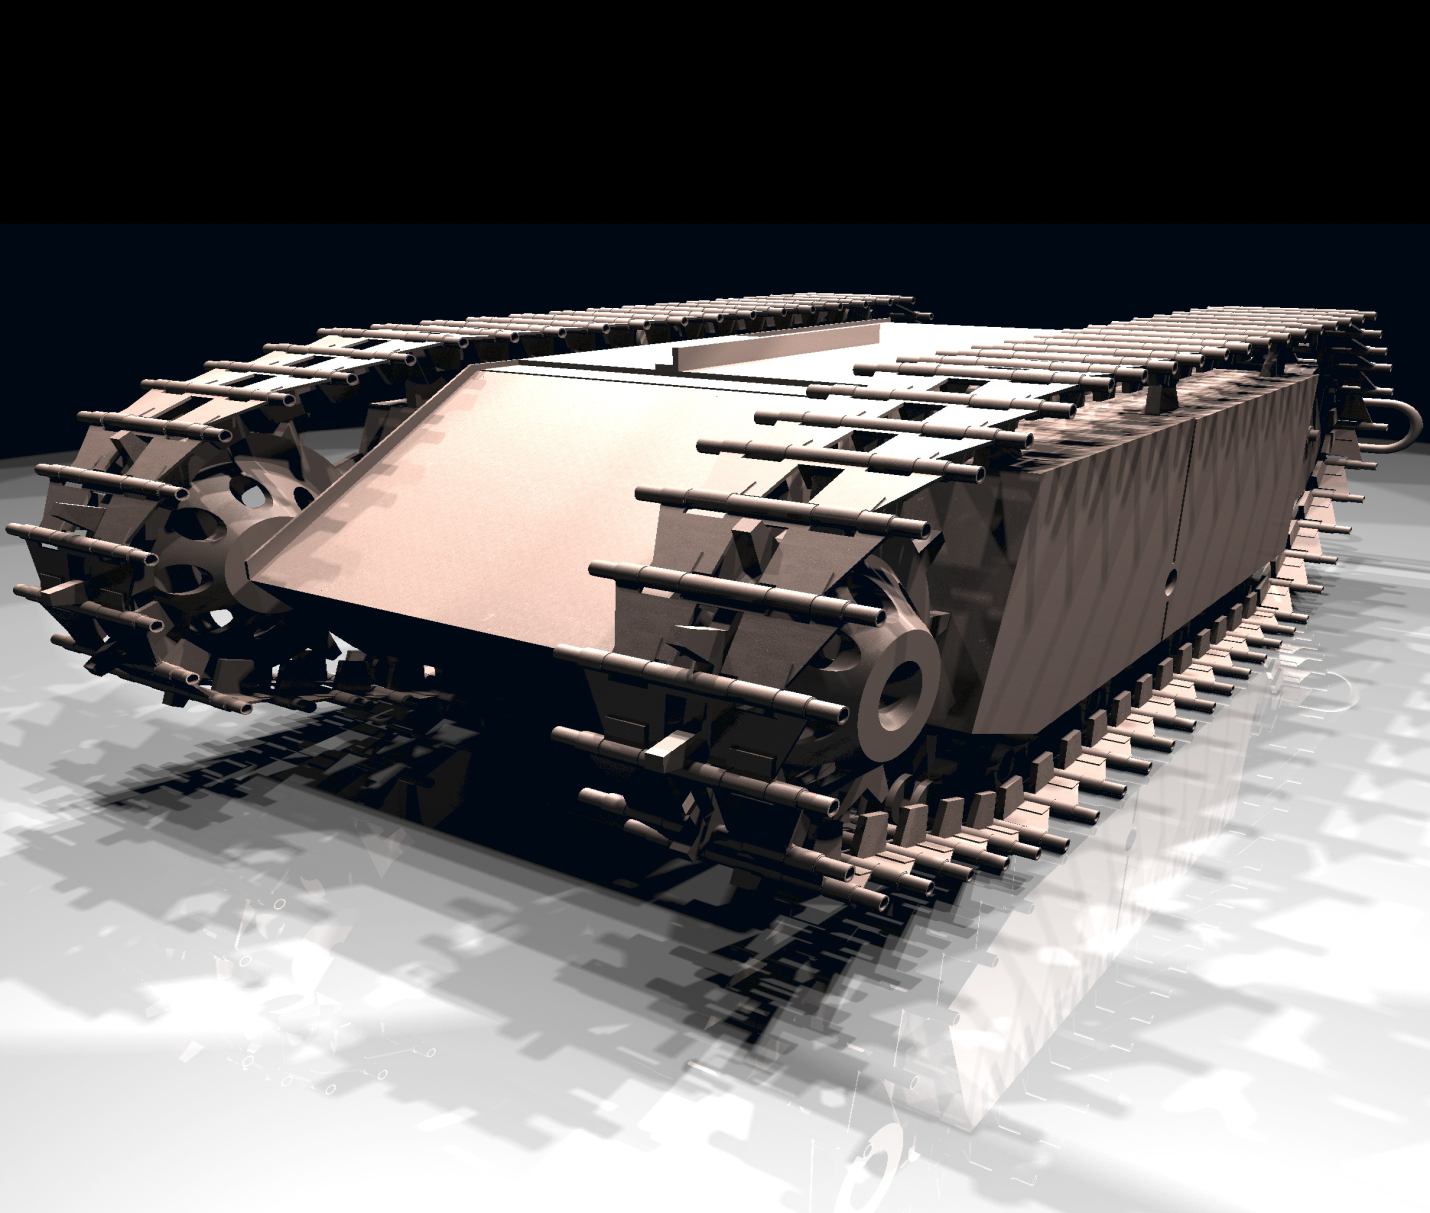
\includegraphics[trim=1cm 2cm 3cm 4cm, clip=true, totalheight=0.5\textheight]{Figures/Goliath.png}
\caption[Model of a Goliath tracked mine]{Model of a Goliath tracked mine}
\label{Goliath}
\end{figure}

%--------------------------------------------------------------------------------------------

\subsection{A (not so short) Introduction to \LaTeX{}}

If you are new to \LaTeX{}, there is a very good eBook -- freely available online as a PDF file -- called, ``The Not So Short Introduction to \LaTeX{}''. The book's title is typically shortened to just ``lshort''. You can download the latest version (as it is occasionally updated) from here:\\
\href{http://www.ctan.org/tex-archive/info/lshort/english/lshort.pdf}{\texttt{http://www.ctan.org/tex-archive/info/lshort/english/lshort.pdf}}

It is also available in several other languages. Find yours from the list on this page:\\
\href{http://www.ctan.org/tex-archive/info/lshort/}{\texttt{http://www.ctan.org/tex-archive/info/lshort/}}

It is recommended to take a little time out to learn how to use \LaTeX{} by creating several, small `test' documents. Making the effort now means you're not stuck learning the system when what you \emph{really} need to be doing is writing your thesis.

\subsection{A Short Math Guide for \LaTeX{}}

If you are writing a technical or mathematical thesis, then you may want to read the document by the AMS (American Mathematical Society) called, ``A Short Math Guide for \LaTeX{}''. It can be found online here:\\
\href{http://www.ams.org/tex/amslatex.html}{\texttt{http://www.ams.org/tex/amslatex.html}}\\
under the ``Additional Documentation'' section towards the bottom of the page.

\subsection{Common \LaTeX{} Math Symbols}
There are a multitude of mathematical symbols available for \LaTeX{} and it would take a great effort to learn the commands for them all. The most common ones you are likely to use are shown on this page:\\
\href{http://www.sunilpatel.co.uk/latexsymbols.html}{\texttt{http://www.sunilpatel.co.uk/latexsymbols.html}}

You can use this page as a reference or crib sheet, the symbols are rendered as large, high quality images so you can quickly find the \LaTeX{} command for the symbol you need.

\subsection{\LaTeX{} on a Mac}
 
The \LaTeX{} package is available for many systems including Windows, Linux and Mac OS X. The package for OS X is called MacTeX and it contains all the applications you need -- bundled together and pre-customised -- for a fully working \LaTeX{} environment and workflow.
 
MacTeX includes a dedicated \LaTeX{} IDE (Integrated Development Environment) called ``TeXShop'' for writing your `\texttt{.tex}' files and ``BibDesk'': a program to manage your references and create your bibliography section just as easily as managing songs and creating playlists in iTunes.

%----------------------------------------------------------------------------------------

\section{Getting Started with this Template}

If you are familiar with \LaTeX{}, then you can familiarise yourself with the contents of the Zip file and the directory structure and then place your own information into the `\texttt{Thesis.cls}' file. Section \ref{FillingFile} on page \pageref{FillingFile} tells you how to do this. Make sure you read section \ref{ThesisConventions} about thesis conventions to get the most out of this template and then get started with the `\texttt{Thesis.tex}' file straightaway.

If you are new to \LaTeX{} it is recommended that you carry on reading through the rest of the information in this document.

\subsection{About this Template}

This \LaTeX{} Thesis Template is originally based and created around a \LaTeX{} style file created by Steve R.\ Gunn from the University of Southampton (UK), department of Electronics and Computer Science. You can find his original thesis style file at his site, here:\\
\href{http://www.ecs.soton.ac.uk/~srg/softwaretools/document/templates/}{\texttt{http://www.ecs.soton.ac.uk/$\sim$srg/softwaretools/document/templates/}}

My thesis originally used the `\texttt{ecsthesis.cls}' from his list of styles. However, I knew \LaTeX{} could still format better. To get the look I wanted, I modified his style and also created a skeleton framework and folder structure to place the thesis files in.

This Thesis Template consists of that modified style, the framework and the folder structure. All the work that has gone into the preparation and groundwork means that all you have to bother about is the writing.

Before you begin using this template you should ensure that its style complies with the thesis style guidelines imposed by your institution. In most cases this template style and layout will be suitable. If it is not, it may only require a small change to bring the template in line with your institution's recommendations.

%----------------------------------------------------------------------------------------

\section{What this Template Includes}

\subsection{Folders}

This template comes as a single Zip file that expands out to many files and folders. The folder names are mostly self-explanatory:

\textbf{Appendices} -- this is the folder where you put the appendices. Each appendix should go into its own separate `\texttt{.tex}' file. A template is included in the directory.

\textbf{Chapters} -- this is the folder where you put the thesis chapters. A thesis usually has about seven chapters, though there is no hard rule on this. Each chapter should go in its own separate `\texttt{.tex}' file and they usually are split as:
\begin{itemize}
\item Chapter 1: Introduction to the thesis topic
\item Chapter 2: Background information and theory
\item Chapter 3: (Laboratory) experimental setup
\item Chapter 4: Details of experiment 1
\item Chapter 5: Details of experiment 2
\item Chapter 6: Discussion of the experimental results
\item Chapter 7: Conclusion and future directions
\end{itemize}
This chapter layout is specialised for the experimental sciences.

\textbf{Figures} -- this folder contains all figures for the thesis. These are the final images that will go into the thesis document.

\textbf{Primitives} -- this is the folder that contains scraps, particularly because one final image in the `Figures' folder may be made from many separate images and photos, these source images go here. This keeps the intermediate files separate from the final thesis figures.

\subsection{Files}

Included are also several files, most of them are plain text and you can see their contents in a text editor. Luckily, many of them are auxiliary files created by \LaTeX{} or BibTeX and which you don't need to bother about:

\textbf{Bibliography.bib} -- this is an important file that contains all the bibliographic information and references that you will be citing in the thesis for use with BibTeX. You can write it manually, but there are reference manager programs available that will create and manage it for you. Bibliographies in \LaTeX{} are a large subject and you may need to read about BibTeX before starting with this.

\textbf{Thesis.cls} -- this is an important file. It is the style file that tells \LaTeX{} how to format the thesis. You will also need to open this file in a text editor and fill in your own information (such as name, department, institution). Luckily, this is not too difficult and is explained in section \ref{FillingFile} on page \pageref{FillingFile}.

\textbf{Thesis.pdf} -- this is your beautifully typeset thesis (in the PDF file format) created by \LaTeX{}.

\textbf{Thesis.tex} -- this is an important file. This is the file that you tell \LaTeX{} to compile to produce your thesis as a PDF file. It contains the framework and constructs that tell \LaTeX{} how to layout the thesis. It is heavily commented so you can read exactly what each line of code does and why it is there. After you put your own information into the `\texttt{Thesis.cls}' file, go to this file and begin filling it in -- you have now started your thesis!

\textbf{vector.sty} -- this is a \LaTeX{} package, it tells \LaTeX{} how to typeset mathematical vectors. Using this package is very easy and you can read the documentation on the site (you just need to look at the `\texttt{vector.pdf}' file):\\
\href{http://www.ctan.org/tex-archive/macros/latex/contrib/vector/}{\texttt{http://www.ctan.org/tex-archive/macros/latex/contrib/vector/}}

\textbf{lstpatch.sty} -- this is a \LaTeX{} package required by this LaTeX template and is included as not all \TeX{} distributions have it installed by default. You do not need to modify this file.

Files that are \emph{not} included, but are created by \LaTeX{} as auxiliary files include:

\textbf{Thesis.aux} -- this is an auxiliary file generated by \LaTeX{}, if it is deleted \LaTeX{} simply regenerates it when you run the main `\texttt{.tex}' file.

\textbf{Thesis.bbl} -- this is an auxiliary file generated by BibTeX, if it is deleted, BibTeX simply regenerates it when you run the main tex file. Whereas the `\texttt{.bib}' file contains all the references you have, this `\texttt{.bbl}' file contains the references you have actually cited in the thesis and is used to build the bibliography section of the thesis.

\textbf{Thesis.blg} -- this is an auxiliary file generated by BibTeX, if it is deleted BibTeX simply regenerates it when you run the main `\texttt{.tex}' file.

\textbf{Thesis.lof} -- this is an auxiliary file generated by \LaTeX{}, if it is deleted \LaTeX{} simply regenerates it when you run the main `\texttt{.tex}' file. It tells \LaTeX{} how to build the `List of Figures' section.

\textbf{Thesis.log} -- this is an auxiliary file generated by \LaTeX{}, if it is deleted \LaTeX{} simply regenerates it when you run the main `\texttt{.tex}' file. It contains messages from \LaTeX{}, if you receive errors and warnings from \LaTeX{}, they will be in this `\texttt{.log}' file.

\textbf{Thesis.lot} -- this is an auxiliary file generated by \LaTeX{}, if it is deleted \LaTeX{} simply regenerates it when you run the main `\texttt{.tex}' file. It tells \LaTeX{} how to build the `List of Tables' section.

\textbf{Thesis.out} -- this is an auxiliary file generated by \LaTeX{}, if it is deleted \LaTeX{} simply regenerates it when you run the main `\texttt{.tex}' file.


So from this long list, only the files with the `\texttt{.sty}', `\texttt{.bib}', `\texttt{.cls}' and `\texttt{.tex}' extensions are the most important ones. The other auxiliary files can be ignored or deleted as \LaTeX{} and BibTeX will regenerate them.

%----------------------------------------------------------------------------------------

\section{Filling in the `\texttt{Thesis.cls}' File}\label{FillingFile}

You will need to personalise the thesis template and make it your own by filling in your own information. This is done by editing the `\texttt{Thesis.cls}' file in a text editor.

Open the file and scroll down, past all the `$\backslash$\texttt{newcommand}\ldots' items until you see the entries for `\texttt{University Name}', `\texttt{Department Name}', etc\ldots.

Fill out the information about your group and institution and ensure you keep to block capitals where it asks you to. You can also insert web links, if you do, make sure you use the full URL, including the `\texttt{http://}' for this.

The last item you should need to fill in is the Faculty Name (in block capitals). When you have done this, save the file and recompile `\texttt{Thesis.tex}'. All the information you filled in should now be in the PDF, complete with web links. You can now begin your thesis proper!

%----------------------------------------------------------------------------------------

\section{The `\texttt{Thesis.tex}' File Explained}

The \texttt{Thesis.tex} file contains the structure of the thesis. There are plenty of written comments that explain what pages, sections and formatting the \LaTeX{} code is creating. Initially there seems to be a lot of \LaTeX{} code, but this is all formatting, and it has all been taken care of so you don't have to do it.

Begin by checking that your information on the title page is correct. For the thesis declaration, your institution may insist on something different than the text given. If this is the case, just replace what you see with what is required.

Then comes a page which contains a funny quote. You can put your own, or quote your favourite scientist, author, person, etc\ldots Make sure to put the name of the person who you took the quote from.

Next comes the acknowledgements. On this page, write about all the people who you wish to thank (not forgetting parents, partners and your advisor/supervisor).

The contents pages, list of figures and tables are all taken care of for you and do not need to be manually created or edited. The next set of pages are optional and can be deleted since they are for a more technical thesis: insert a list of abbreviations you have used in the thesis, then a list of the physical constants and numbers you refer to and finally, a list of mathematical symbols used in any formulae. Making the effort to fill these tables means the reader has a one-stop place to refer to instead of searching the internet and references to try and find out what you meant by certain abbreviations or symbols.

The list of symbols is split into the Roman and Greek alphabets. Whereas the abbreviations and symbols ought to be listed in alphabetical order (and this is \emph{not} done automatically for you) the list of physical constants should be grouped into similar themes.

The next page contains a one line dedication. Who will you dedicate your thesis to?

Finally, there is the section where the chapters are included. Uncomment the lines (delete the `\texttt{\%}' character) as you write the chapters. Each chapter should be written in its own file and put into the `Chapters' folder and named `\texttt{Chapter1}', `\texttt{Chapter2}, etc\ldots Similarly for the appendices, uncomment the lines as you need them. Each appendix should go into its own file and placed in the `Appendices' folder.

After the preamble, chapters and appendices finally comes the bibliography. The bibliography style (called `\texttt{unsrtnat}') is used for the bibliography and is a fully featured style that will even include links to where the referenced paper can be found online. Do not under estimate how grateful you reader will be to find that a reference to a paper is just a click away. Of course, this relies on you putting the URL information into the BibTeX file in the first place.

%----------------------------------------------------------------------------------------

\section{Thesis Features and Conventions}\label{ThesisConventions}

To get the best out of this template, there are a few conventions that you may want to follow.

One of the most important (and most difficult) things to keep track of in such a long document as a thesis is consistency. Using certain conventions and ways of doing things (such as using a Todo list) makes the job easier. Of course, all of these are optional and you can adopt your own method.

\subsection{Printing Format}

This thesis template is designed for single sided printing as most theses are printed and bound this way. This means that the left margin is always wider than the right (for binding). Four out of five people will now judge the margins by eye and think, ``I never 
noticed that before.''.

The headers for the pages contain the page number on the right side (so it is easy to flick through to the page you want) and the chapter name on the left side.

The text is set to 11 point and a line spacing of 1.3. Generally, it is much more readable to have a smaller text size and wider gap between the lines than it is to have a larger text size and smaller gap. Again, you can tune the text size and spacing should you want or need to. The text size can be set in the options for the `$\backslash$\texttt{documentclass}' command at the top of the `\texttt{Thesis.tex}' file and the spacing can be changed by setting a different value in the `$\backslash$\texttt{setstretch}' commands (scattered throughout the `\texttt{Thesis.tex}' file).

\subsection{Using US Letter Paper}

The paper size used in the template is A4, which is a common -- if not standard -- size in Europe. If you are using this thesis template elsewhere and particularly in the United States, then you may have to change the A4 paper size to the US Letter size. Unfortunately, this is not as simple as replacing instances of `\texttt{a4paper}' with `\texttt{letterpaper}'.

This is because the final PDF file is created directly from the \LaTeX{} source using a program called `\texttt{pdfTeX}' and in certain conditions, paper size commands are ignored and all documents are created with the paper size set to the size stated in the configuration file for pdfTeX (called `\texttt{pdftex.cfg}').

What needs to be done is to change the paper size in the configuration file for \texttt{pdfTeX} to reflect the letter size. There is an excellent tutorial on how to do this here: \\
\href{http://www.physics.wm.edu/~norman/latexhints/pdf_papersize.html}{\texttt{http://www.physics.wm.edu/$\sim$norman/latexhints/pdf\_papersize.html}}

It may be sufficient just to replace the dimensions of the A4 paper size with the US Letter size in the \texttt{pdftex.cfg} file. Due to the differences in the paper size, the resulting margins may be different to what you like or require (as it is common for Institutions to dictate certain margin sizes). If this is the case, then the margin sizes can be tweaked by opening up the \texttt{Thesis.cls} file and searching for the line beginning with, `$\backslash$\texttt{setmarginsrb}' (not very far down from the top), there you will see the margins specified. Simply change those values to what you need (or what looks good) and save. Now your document should be set up for US Letter paper size with suitable margins.

\subsection{References}

The `\texttt{natbib}' package is used to format the bibliography and inserts references such as this one \citep{Reference3}. The options used in the `\texttt{Thesis.tex}' file mean that the references are listed in numerical order as they appear in the text. Multiple references are rearranged in numerical order (e.g. \citep{Reference2, Reference1}) and multiple, sequential references become reformatted to a reference range (e.g. \citep{Reference2, Reference1, Reference3}). This is done automatically for you. To see how you use references, have a look at the `\texttt{Chapter1.tex}' source file. Many reference managers allow you to simply drag the reference into the document as you type.

Scientific references should come \emph{before} the punctuation mark if there is one (such as a comma or period). The same goes for footnotes\footnote{Such as this footnote, here down at the bottom of the page.}. You can change this but the most important thing is to keep the convention consistent throughout the thesis. Footnotes themselves should be full, descriptive sentences (beginning with a capital letter and ending with a full stop).

To see how \LaTeX{} typesets the bibliography, have a look at the very end of this document (or just click on the reference number links).

\subsection{Figures}

There will hopefully be many figures in your thesis (that should be placed in the `Figures' folder). The way to insert figures into your thesis is to use a code template like this:
\begin{verbatim}
\begin{figure}[htbp]
  \centering
    
\includegraphics{Figures/Electron.pdf}
    \rule{35em}{0.5pt}
  \caption[An Electron]{An electron (artist's impression).}
  \label{fig:Electron}
\end{figure}
\end{verbatim}
Also look in the source file. Putting this code into the source file produces the picture of the electron that you can see in the figure below.

\begin{figure}[htbp]
	\centering
		
\includegraphics{Figures/Electron.pdf}
		\rule{35em}{0.5pt}
	\caption[An Electron]{An electron (artist's impression).}
	\label{fig:Electron}
\end{figure}

Sometimes figures don't always appear where you write them in the source. The placement depends on how much space there is on the page for the figure. Sometimes there is not enough room to fit a figure directly where it should go (in relation to the text) and so \LaTeX{} puts it at the top of the next page. Positioning figures is the job of \LaTeX{} and so you should only worry about making them look good!

Figures usually should have labels just in case you need to refer to them (such as in Figure \ref{fig:Electron}). The `$\backslash$\texttt{caption}' command contains two parts, the first part, inside the square brackets is the title that will appear in the `List of Figures', and so should be short. The second part in the curly brackets should contain the longer and more descriptive caption text.

The `$\backslash$\texttt{rule}' command is optional and simply puts an aesthetic horizontal line below the image. If you do this for one image, do it for all of them.

The \LaTeX{} Thesis Template is able to use figures that are either in the PDF or JPEG file format.

\subsection{Typesetting mathematics}

If your thesis is going to contain heavy mathematical content, be sure that \LaTeX{} will make it look beautiful, even though it won't be able to solve the equations for you.

The ``Not So Short Introduction to \LaTeX{}'' (available \href{http://www.ctan.org/tex-archive/info/lshort/english/lshort.pdf}{here}) should tell you everything you need to know for most cases of typesetting mathematics. If you need more information, a much more thorough mathematical guide is available from the AMS called, ``A Short Math Guide to \LaTeX{}'' and can be downloaded from:\\
\href{ftp://ftp.ams.org/pub/tex/doc/amsmath/short-math-guide.pdf}{\texttt{ftp://ftp.ams.org/pub/tex/doc/amsmath/short-math-guide.pdf}}

There are many different \LaTeX{} symbols to remember, luckily you can find the most common symbols \href{http://www.sunilpatel.co.uk/latexsymbols.html}{here}. You can use the web page as a quick reference or crib sheet and because the symbols are grouped and rendered as high quality images (each with a downloadable PDF), finding the symbol you need is quick and easy.

You can write an equation, which is automatically given an equation number by \LaTeX{} like this:
\begin{verbatim}
\begin{equation}
E = mc^{2}
  \label{eqn:Einstein}
\end{equation}
\end{verbatim}

This will produce Einstein's famous energy-matter equivalence equation:
\begin{equation}
E = mc^{2}
\label{eqn:Einstein}
\end{equation}

All equations you write (which are not in the middle of paragraph text) are automatically given equation numbers by \LaTeX{}. If you don't want a particular equation numbered, just put the command, `$\backslash$\texttt{nonumber}' immediately after the equation.

%----------------------------------------------------------------------------------------

\section{Sectioning and Subsectioning}

You should break your thesis up into nice, bite-sized sections and subsections. \LaTeX{} automatically builds a table of Contents by looking at all the `$\backslash$\texttt{chapter}$\{\}$', `$\backslash$\texttt{section}$\{\}$' and `$\backslash$\texttt{subsection}$\{\}$' commands you write in the source.

The table of Contents should only list the sections to three (3) levels. A `$\backslash$\texttt{chapter}$\{\}$' is level one (1). A `$\backslash$\texttt{section}$\{\}$' is level two (2) and so a `$\backslash$\texttt{subsection}$\{\}$' is level three (3). In your thesis it is likely that you will even use a `$\backslash$\texttt{subsubsection}$\{\}$', which is level four (4). Adding all these will create an unnecessarily cluttered table of Contents and so you should use the `$\backslash$\texttt{subsubsection$^{*}\{\}$}' command instead (note the asterisk). The asterisk ($^{*}$) tells \LaTeX{} to omit listing the subsubsection in the Contents, keeping it clean and tidy.

%----------------------------------------------------------------------------------------

\section{In Closing}

You have reached the end of this mini-guide. You can now rename or overwrite this pdf file and begin writing your own `\texttt{Chapter1.tex}' and the rest of your thesis. The easy work of setting up the structure and framework has been taken care of for you. It's now your job to fill it out!

Good luck and have lots of fun!

\begin{flushright}
Guide written by ---\\
Sunil Patel: \href{http://www.sunilpatel.co.uk}{www.sunilpatel.co.uk}
\end{flushright}

% Chapter 2

\chapter{LITERATURE REVIEW OF GEOMETRIC MODELING} % Main chapter title

\label{Literature Review} % Change X to a consecutive number; for referencing this chapter elsewhere, use \ref{ChapterX}

\lhead{Chapter 2. \emph{Literature Review}} % Change X to a consecutive number; this is for the header on each page - perhaps a shortened title

%----------------------------------------------------------------------------------------
%      INTRODUCTORY PARAGRAPHS
%----------------------------------------------------------------------------------------
\hspace{30} With the advent of computers which could perform millions of floating
point operations in unit time and which are still growing faster, researchers who
believed computers could aid the processes of mechanical design and
manufacturing were faced with a critical issue – how to represent physical
reality using computer software. They sought the best data structures to
represent this reality and the most appropriate algorithms to manipulate these representations.

\hspace{30} BRL-­CAD supports a wide variety of geometric representations including an 
extensive set of traditional implicit primitive shapes as well as explicit primitives
made from collections of uniform B­spline surfaces, non­uniform rational B­spline (NURBS)
surfaces, n­on-manifold   geometry   (NMG)   and purely faceted polygonal mesh geometry.
Consequently, in this chapter, we review the existing work done by scholars in the 
field of geometric modeling which have been applied to the development of BRL-­CAD. 
First of all, it introduces the issue of representation and the notion of representation
 schemes.Then, it summarizes developments in wireframe modeling, surface modeling, solid
modeling and non­-manifold modeling (aka non­manifold geometry or nmg for short) with a keen
 eye on the algorithms underlying them.

\hspace{30} As we progress in our literature review from older forms of geometric
modeling to newer ones, we will discover that representation schemes were
closely linked to algorithmic efficiency and that it has always been normal to
expect designers to switch to newer ones in response to the improvements in
algorithmic performance.Despite these enhancements in algorithmic efficiency
within the designer community, we cannot say with complete certainty whether
traditional representation schemes can be relegated to the background. We
can only conclude that old and new representation paradigms co­exist and that
research led to representation schemes which supplemented the repertoire of
geometric modeling.  

%-----------------------------------------------------------------------------------------

%----------------------------------------------------------------------------------------
%	SECTION 1
%----------------------------------------------------------------------------------------

\section{Representation Schemes}

A representation $\textbf{\mathfrak{R}}$ of a solid or representation for short is a subset of
three­-dimensional Euclidean space denoted $\mathbb{E}^3$ which models a physical solid.  
According to [5], Requicha and Tilove stated that point set topology provided a
formal language for describing the geometric properties of solids and they also  
threw more light on the mathematical characteristics of solids such as a solid's
interior, boundary, complement, closure, boundedness and regularity.
Requicha [4] insisted that to be computationally useful, a representation should  
formally capture the following properties ;

%-----------------------------------
%	SUBSECTION 1
%-----------------------------------
\subsection{Subsection 1}

Nunc posuere quam at lectus tristique eu ultrices augue venenatis. Vestibulum ante ipsum primis in faucibus orci luctus et ultrices posuere cubilia Curae; Aliquam erat volutpat. Vivamus sodales tortor eget quam adipiscing in vulputate ante ullamcorper. Sed eros ante, lacinia et sollicitudin et, aliquam sit amet augue. In hac habitasse platea dictumst.

%-----------------------------------
%	SUBSECTION 2
%-----------------------------------

\subsection{Subsection 2}
Morbi rutrum odio eget arcu adipiscing sodales. Aenean et purus a est pulvinar pellentesque. Cras in elit neque, quis varius elit. Phasellus fringilla, nibh eu tempus venenatis, dolor elit posuere quam, quis adipiscing urna leo nec orci. Sed nec nulla auctor odio aliquet consequat. Ut nec nulla in ante ullamcorper aliquam at sed dolor. Phasellus fermentum magna in augue gravida cursus. Cras sed pretium lorem. Pellentesque eget ornare odio. Proin accumsan, massa viverra cursus pharetra, ipsum nisi lobortis velit, a malesuada dolor lorem eu neque.

%----------------------------------------------------------------------------------------
%	SECTION 2
%----------------------------------------------------------------------------------------

\section{Main Section 2}

Sed ullamcorper quam eu nisl interdum at interdum enim egestas. Aliquam placerat justo sed lectus lobortis ut porta nisl porttitor. Vestibulum mi dolor, lacinia molestie gravida at, tempus vitae ligula. Donec eget quam sapien, in viverra eros. Donec pellentesque justo a massa fringilla non vestibulum metus vestibulum. Vestibulum in orci quis felis tempor lacinia. Vivamus ornare ultrices facilisis. Ut hendrerit volutpat vulputate. Morbi condimentum venenatis augue, id porta ipsum vulputate in. Curabitur luctus tempus justo. Vestibulum risus lectus, adipiscing nec condimentum quis, condimentum nec nisl. Aliquam dictum sagittis velit sed iaculis. Morbi tristique augue sit amet nulla pulvinar id facilisis ligula mollis. Nam elit libero, tincidunt ut aliquam at, molestie in quam. Aenean rhoncus vehicula hendrerit.
 
%------------------------------------------------------------------------------------------------
\chapter{ANALYSIS \& DESIGN}
\label{Analysis \& Design}
\lhead{Chapter 3. \emph{Analysis \& Design}}
%----------------------------------------------------------------------------------------
%	SECTION 1
%----------------------------------------------------------------------------------------

\hspace{30} In this chapter,   we   state   our   aim   of   contributing   to   the   BRL-­CAD   project  
and   explain   how   we   implemented   a   heart-shaped   primitive   in   the   project   design  
section.   Firstly,   we   introduce   the   concept   of   free   and   open   source   software. Secondly,   we   do   an   overview   of   the   BRL-­CAD   software   package.   After,   we  state   our   aim   of   contributing   to   the   BRL-­CAD   project.   Finally,   we   give   a   detailed  explanation   of   the   design   which   we   employed   to   implement   the   heart-­shaped primitive for BRL-CAD.

%------------------------------------------------------------------------------------------------------------------------------
%		OPEN SOURCE COMMUNITY
%------------------------------------------------------------------------------------------------------------------------------
\section{The Open Source Community}

\hspace{30} Depending   on   how   we   choose   to   call   it,   \textit{Free/Libre/Open   Source  
Software   (FLOSS)},   \textit{Free   and   Open   Source   Software   (FOSS)}   or   simply   \textit{Open  
Source   Software   OSS)}   is   software   for   which   users   have   access   to   both   the  
source   code   and   binary   executables   and   is   licensed   under   a   license   which  
permits   its   users   to   read,   edit   and   distribute   the   software   to   anyone   and   for   any  
reason.   This   distinguishes   open   source   software   from   commercial   software  
which   is   distributed   by   giving   away   its   binary   executable   version   only.   Usually,  
OSS   is   distributed   at   no   cost   with   limited   restrictions   on   how   it   can   be   used.  
According   to   Eric   S.   Raymond \cite{33},   one   of   the   most   prominent   evangelists   of  
the   open   source   movement,   hackerdom   can   be   likened   to   what   anthropologists  
call   a   gift   culture–   a   culture   wherein   members   gain   status   and   reputation   by  
giving   away   their   time,   creativity   and   skills   to   reading,   writing   and   debugging  
software,   publishing   useful   information   in   blogs   or   documents   like   Frequently  
Asked   Questions   (FAQs)   lists   as   well   as   handling   unglamorous   tasks   like  
maintaining   mailing   lists,   moderating   news   groups,   etc   without   any   monetary  
compensation.   The   word   \textit{\textbf{hacker}}   was   coined   by   a   shared   community   of   expert  
programmers   and   networking   masters   which   traces   its   history   back   to   the   days  
of   the   earliest   ARPAnet   experiments   and   time­sharing   minicomputers   who  
made   the   unix   operating   systems   and   the   world­wide   web   work.   As   opposed   to  
hackers,   \textit{\textbf{crackers}}   who   are   more   interested   in   breaking   software   and   perturbing  
phone systems.   

\hspace{30} Today,   the   open   source   community   has   become   a   self­organizing  
collaborative   social   network   of   hackers   driven   by   a   passion   to   solve   problems  
using   free   software   with   thousands   of   projects   hosted   on   Sourceforge \cite{34}   and  
Github \cite{35}.   It   has   singularly   developed   some   software   packages   and   tools  
which   are   the   best   in   the   world   such   as   the   firefox   web   browser,   Apache  
web­server,   Linux   operating   systems   like   BSD,   Ubuntu,   Debian, etc,   the   MySQL  
database   management   system,   the   VLC   media   player,   programming  languages   and   tools   like   gcc,   C,   Perl,   Python,   Java,   etc   and   much   more.   Some  Examples   of   CAD   packages   within   the   open   source  community   include   BRL­-CAD,   Blender,   FreeCAD,   OpenSCAD   and   LibreCAD,  
etc.

%--------------------------------------------------------------------------------------------------------------------------------

%--------------------------------------------------------------------------------------------------------------------------------
%	ANALYSIS OF THE WORK
%--------------------------------------------------------------------------------------------------------------------------------
\section{Analysis Of The Work}

\hspace{30} BRL­-CAD   (   pronounced   Be­-Are-­El-­CAD)   was   originally   conceived   and  
written   by   the   late   Mike   Muss,   a   programmer   and   networking   expert   who   also  
wrote   the   popular   PING   network   program.   In   1979,   the   United   States   Army's  
Ballistic   Research   Laboratory   (BRL)   (the   agency   responsible   for   creating  
ENIAC,   the   world's   first   general-­purpose   electronic   computer   in   the   1940s)  
identified   a   need   for   tools   that   could   assist   with   the   computer   simulations   and  
analysis   of   combat   vehicle   systems   and   environments.   When   no   existing   CAD  
package   was   found   to   be   adequate   for   this   specialized   purpose,   Mike   and  
fellow   software   developers   began   developing   and   assembling   a   unique   suite   of  
utilities   capable   of   interactively   displaying,   editing,   and   interrogating   geometric  
models.   Those   early   efforts   subsequently   became   the   foundation   on   which  
BRL­-CAD was built.  

\hspace{30} The   initial   architecture   and   design   of   BRL-­CAD   began   in   1979   and   its  
development   as   a   unified   software   package   kicked   off   in   1983   with   its   first  
public   release   the   following   year.   As   a   software   package   with   a   mature   code  
base   which   has   been   actively   developed   for   decades,   BRL-­CAD   pays   close  
attention   to   design   and   maintainability.   Like   other   FLOSS   packages,  
BRL­-CAD's   source   code   and   most   of   its   project   data   are   stored   in   a  
subversion   version   control   system   for   change   tracking,   collaborative  
development   and   is   redistributed   as   free   and   open   source   software   under   the  
Open   Source   Initiative   license   terms.   The   design   of   its   system   architecture   is  
based   on   a   UNIX­ methodology   of   command   of   the   command ­line   services,  
providing   many   tools   that   work   in   harmony   to   complete   a   specific   task.   These  
tools   include   geometry   and   image   converters,signal   and   image   processing  
tools,   various   ray   tracing   applications, geometry   manipulators,   and   much   more.  
They   will   also   be   used   to   test   that   the   geometric   properties   of   the   heart-­shaped  
primitive works as we will see in Chapter Four.

\hspace{30} The   basic   layout   of   its   code   places   public   API   headers   in   the   top­level  
\textit{\textbf{include/}}   directory   and   source   code   for   both   applications   and   libraries   in   the  
\textit{\textbf{src/}}   directory.   The   following   is   a   partial   listing   of   how   BRL-­CAD's   source   code  
is organised in a typical checkout or source distribution. 

\textbf{Applications and Resources}  

\begin{itemize} 
\item✦ \textit{\textbf{db/}} for Example Geometry.  
\item✦ \textit{\textbf{doc/}} for project Documentation.  
\item✦ \textit{\textbf{include/}} for Public API headers.  
\item✦ \textit{\textbf{regress/}} for Regression test scripts  
\item✦ \textit{\textbf{src/}} for Application and library source.  
\item✦ \textit{\textbf{src/conv}} for Geometry converters.  
\item✦ \textit{\textbf{src/fb}} for Displaying data in windows.  
\item✦ \textit{\textbf{src/mged}} for the Multi­device geometry editor, the main GUI application.   
\item✦ \textit{\textbf{src/rt}} for Ray tracing applications.  
\item✦ \textit{\textbf{src/util}} for Image processing utilities.
\end{itemize}  

\textbf{Libraries}
  
\begin{itemize} 
\item✦ \textit{\textbf{src/libbn}} for Numerics library.  
\item✦ \textit{\textbf{src/libbu}} for Utility library.  
\item✦ \textit{\textbf{src/libgcv}} for Geometry conversion library.  
\item✦ \textit{\textbf{src/libged}} for Geometry Editing library.  
\item✦ \textit{\textbf{src/icv}} for Image conversion library.  
\item✦ \textit{\textbf{src/libpkg}} for Network Package library.  
\item✦ \textit{\textbf{src/librt}} for Ray­tracing library.  
\item✦ \textit{\textbf{src/libwbd}} for Geometry creation library.
\end{itemize}

\hspace{30} The   majority   of   BRL-­CAD's   source   code   is   written   in   ANSI/POSIX   C   with   the  
intent   of   strictly   conforming   with   the   C   standard.   The   core   libraries   are   all   C   API  
though   several   such   as   the   Utility   and   Ray­tracing   libraries   use   C++   for  
implementation   details.   Major   components   of   the   system   are   written   in   C,   C++,  
Tcl/Tk,   Bash   and   PHP   with   source   code   files   using   extensions   such   as   *.c,   *.h,  
*.cpp,   *.tcl,   *.tk,   *.sh   and   *.php.   BRL­CAD   uses   the   CMake   build   system   for  
compilation and an in built testing infrastructure in \textit{\textbf{regress/}} for unit testing.  

\hspace{30} BRL-­CAD   has   a   long­lasting   heritage   of   maintaining   verifiable,   validated  
and   repeatable   results   in   critical   portions   of   the   software   package,   particularly  
within   the   ray   tracing   library.   It   has   an   in built   testing   infrastructure   which  
compares   all   program   output   against   benchmark   results   during   each   build.   The  
ray   tracing   library   is   a   multi­-representational   library   which   lies   at   the   heart   of  
BRL­-CAD   and   uses   a   suite   of   other   libraries   for   other   basic   application  
functionality.   Considerable   attention   is   put   into   verification   and   validation  
throughout   the   package   which   includes   regression   tests   that   compare   runtime  
behaviour   against   known   results   and   reports   any   adverse   variances   from  
standard results as failures.  

\hspace{30} Despite   this   sophisticated   infrastructure,   performant   design   and  
long­lasting   heritage,   many   still   coin   BRL-­CAD's   aspiration   of   one   day   being   the  
most   widely   used   open   source   CAD   package   as   rather   lofty  
for the following reasons;

\begin{itemize}
\item With   one   of   the   fastest   ray­tracers   in   existence   (on   several   types   of  
geometry)   which   is   supported   by   an   effective   Laguerre-­based   root   solver  
and   used   within   academia   for   scientific   instruction,   computer   graphics  
education   and   research,   the   stability   of   BRL­-CAD's   root   solver   on  
higher ­order   polynomials   such   as   quintics   (of   power   5)   and   sextics   (of  
power 6) is still uncertain.

\item As   an   open   source   CAD   software   which   is   deeply   rooted   in   the  
Constructive   Solid   Geometry,   BRL-­CAD's   set   of   primitives   is   still   limited  
to traditional ones such as cones, cylinders, spheres, tori, etc.

\item BRL­-CAD   is   widely   used   within   agencies   within   the   United   States  
Government   for   the   modeling   of   military   artillery   and   simulating   combat  vehicle   systems   and   environments.   This   severely   limits   is   user   base   to  the   military   sector   and   gives   it   an   “­warring”   flare   which   repels   users   who  would have used it for more entertainment purposes.
\end{itemize}

In   a   bid   to   solve   the   aforementioned   problems,   we   embarked   on   a   journey   to  
develop   a   heart-­shaped   primitive   for   BRL­-CAD.   In   the   following   section,   we  
document   how   we   wrote   various   callback   functions   which   compute   useful  
geometric   properties   for   the   heart-­shaped   primitive   such   as   formatted  
description,   database   importation   and   exportation,   computation   of   the   bounding  
box, plotting the wireframe and ray tracing.

%---------------------------------------------------------------------------------------------------------------------------------
%	DESIGN
%---------------------------------------------------------------------------------------------------------------------------------

\section{Design}

\hspace{30} After   having   stated   our   goal   of   contributing   to   the   BRL-­CAD   project,   we  
now   explain   how   we   implemented   the   heart­-shaped   primitive.   Currently,  
BRL­-CAD   aspires   to   become   the   most   widely   used   open   source  
CAD   software   package   in   existence.   Presently,   it   is   mostly  
used   by   the   United   States   of   America's   Government   agencies   which   fund   its  
development   as   well   as   academic   institutes   which   use   use   it   for   computer  
graphics   educations   and   scientific   research.   Aljazeera   news   Channel's   recent  
revelation   that   less   than   1\%   of   the   world's   population   works   in   the   military   sector  
is   indicative   of   the   fact   that   BRL-­CAD's   usage   must   go   beyond   the   military  
sector to break the status­ quo.   

\hspace{30} In   a   bid   to   increase   BRL-­CAD's   user   base   by   inviting   designers   and  
artists   from   the   entertainment   industry,   we   thought   of   developing   a  
heart-­shaped   primitive.   This   heart­-shaped   primitive   (or   simply   heart),   a   symbol  
of   romantic   love,   would   go   a   long   way   to   entertain   families   and   communities  
weddings,   marriage   anniversaries,   valentine's   day   celebrations,   etc.   It   would  
also   be   used   by   fashion   designers   to   create   magnificient   embroidery   on  
clothing.   Lastly,   it   would   also   be   used   to   design   banners   and   royal   coat   of   arms  
in cartoons movies as well as animate embroidery on clothing.   

\hspace{30} While   adhering   to   its   coding   style,   we   incorporated   the   heart-­shaped  
primitive into BRL­-CAD's ray tracing library using the following steps;  

\begin{itemize}
\item We made room for the heart-shaped primitive in BRL­-CAD by hooking it unto the raytracing library.  
\item Wrote callback   functions   for   the   heart   and   tested   them   using   BRL-­CAD's  
inbuilt testing infrastructure in the \textit{\textbf{regress/}} directory.  
\item Built   support   for   typing   in   parameters   for   the   heart-­shaped   primitive   in   the  
display interfaces viz \textit{mged} or \textit{archer}.
\end{itemize}

In   order   to   make   room   for   the   heart­-shape   in   BRL-­CAD,   we   tagged   the   heart  
primitive,   designed   a   data   structure   for   it   and   stubbed   a   skeletal   \textit{hrt.c}   file   into  
the source code repository in \textbf{\textit{src/librt/primitives/hrt/hrt.c.}}

\subsection{Tagging the heart­-shaped primitive}

Given   that   each   of   the   primitives   in   Figure   2.2   above   is   uniquely   stored   in  
BRL-­CAD's   database,   it   was   necessary   to   tag   the   incoming   heart-­shaped  
primitive   with   a   unique   magic   number,   \textbf{Ox6872743f},   which   is   the   hexadecimal  
equivalent   of   “?hrt?”   and   increment   the   maximum   number   of   primitives   in  
\textbf{\textit{src/libbu/magic.c}}, \textbf{\textit{include/magic.h}} and \textbf{\textit{include/raytrace.h}}.  

\subsection{Data Structure of Heart-shaped primitive }

\hspace{30} The   heart-­shape   has   two   lobes   which   are   symmetric   about   the   z­axis   and  
meet at each of its two cusps as the picture in Figure 3.1 shows.  

\begin{figure}[htbp]
\centering
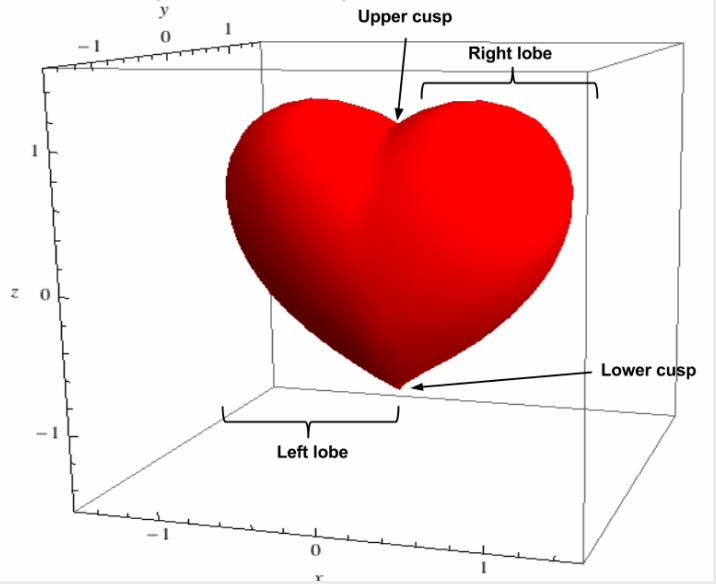
\includegraphics[trim=0.0cm 0.5cm 0.1cm 0.1cm, clip=true, totalheight=0.4\textheight]{Pictures/Heart.png}
\caption[Diagram of the heart-shaped primitive]{Diagram of the heart-shaped primitive}
\label{Heart}
\end{figure}

The   heart-­shape   was   stored   in   the   \textit{\textbf{include/}rtgeom.h}   file   as   an   Abstract   Data  
Type   ( C-­like   structure )   called   \textit{rt\_hrt\_internal}   with   the   following   fields  
representing its parameters.
\begin{itemize}  
\item A magic number \textit{\textbf{hrt\_magic }} 
\item A center point \textit{\textbf{v }} 
\item A vector in the direction of the X-­axis \textit{\textbf{xdir}}  
\item A vector in the directions of the Y­-axis \textit{\textbf{ydir}}  
\item A vector in the direction of the Z­-axis \textit{\textbf{zdir}}  
\item Distance from center point to either cusps \textit{\textbf{d}} 
\end{itemize} 
These   3    vectors viz \textit{\textbf{xdir}}, \textit{\textbf{ydir}} and \textit{\textbf{zdir}}   are   also   called   radial   vectors   because   they   radiate   in   the  X,   Y   and   Z   directions   and   the   aforementioned   structure   is   also   known   in  BRL-­CAD's parlance as the heart-­shape's internal format.

\subsection{A bare bones heart­-shape}

The   signatures   of   the   functions   which   are   called   to   compute   the  
geometric   properties   for   the   heart-­shaped   primitive   were   casted   and   enlisted   in  
a   function   table   in   \textit{src/librt/primitives/table.c}.   Then,   we   added   the  
\textit{src/librt/primitives/hrt/}   directory   to   the   source   code   repository   and   committed  
the   hrt.c   file   to   it.   The   \textit{hrt.c}   file   consisted   of   introductory   comments,   include  
files,   structures   for   raytracing   and   storage   of   the   heart­-shaped   primitive   in   the  
database   as   well   as   stubs   for   all   callback   functions   which   all   print   a  
\textit{\textbf{\“rt\_hrt\_???:Not   implemented   yet!\”}}   message   when   called.   For   surface  
representation   and   raytracing   reasons,   the   heart-­shape   is   stored   in   a   more  
elaborate C-­like structure called \textit{hrt\_specific} with the following parameters;  

\begin{itemize}
\item A position vector for the heart-shape's center \textbf{\textit{hrt\_V}}  
\item A unit vector in the X ­axis direction \textbf{\textit{hrt\_X}}  
\item A unit vector in the Y axis direction \textbf{\textit{hrt\_Y}}  
\item A unit vector in the Z axis direction \textbf{\textit{hrt\_Z}}  
\item A unit vector in the Z ­axis direction \textit{\textbf{hrt\_d}}  
\item A matrix for scaling and rotating \textit{\textbf{hrt\_SoR}}  
\item A matrix for scaling and transposing a rotated heart \textbf{\textit{hrt\_invRSSR}}  
\item A matrix for transposing a rotated heart \textit{\textbf{hrt\_invR}}  
\item A vector for the inverse of the squared magnitudes of the three (3) aforementioned unit vectors \textit{\textbf{hrt\_invsq}}  
\end{itemize}

The   location   of   the   \textit{hrt.c}   file   in   the   raytracing   library   was   added   to  
\textit{src/librt/CMakeLists.txt} for compilation purposes  and test ­driven development.\\
   
\hspace{30} After   hooking   the   heart-­shaped   primitive   into   BRL-­CAD's   source   code  
repository,   we   wrote   callback   functions   which   compute   geometrically   useful  
properties for the primitive such as;   

\begin{enumerate}
\item Formatted description  
\item Database importation and exportation  
\item Computing the bounding box of the heart­-shaped primitive  
\item Plotting the wireframe of the heart­-shaped primitive  
\item Implicit surface representation of the heart-­shaped primitive  
\end{enumerate}

\hspace{30} We   now   explain   how   the   functions   we   wrote   actually   compute   each
of   these properties.   Each   property   was   tested   using   BRL-­CAD's   commands \cite{36}   after  having   
written   the   requisite   function(s)   that   compute   it.   It   is   worth   highlighting  
here   that   the   \textit{“rt\_hrt\_”}   prefix   is   attached   to   the   heart­-shaped   primitive's   structure  
and   its   functions'   signatures   because   \textit{“rt”}   and   \textit{“hrt”}   denote   the   raytracing   library  
and the heart-shape respectively.  

\subsection{Formatted description of the heart­-shaped primitive}

\hspace{30} It   often   arises   that   engineers   and   scientists   working   on   geometric   models  
ask   to   know   the   exact   values   of   the   objects   in   question.   In   order   to   know   a  
solid's   type   and   the   values   of   its   key   parameters,   we   wrote   the   \textit{rt\_hrt\_describe()}  
function   which   simply   prints   the   heart-shape's   parameters   in   human   readable   format.  
The   radial   vectors   in   the   X,   Y   and   Z   directions   are   printed   alongside   their  
magnitudes   and   the   distance   from   the   heart-shape's   center   to   either   of   its   cusps   is  
also printed.

\subsection{Database importation and exportation of the heart­-shaped primitive}

\hspace{30} BRL-­CAD   provides   CSG   modeling   features   and   its   models   are   usually  
stored   in   it's   Geometric   Editing   database   called   GED.   For   the   heart­shaped  
primitive   to   be   used   in   CSG,   we   wrote   functions   that  
import and export data in between the database format and the internal format. 
  
The   \textit{rt\_hrt\_import5()}   function   imports   a   heart   from   the   database   format   to   the  
internal   format.   Firstly,   we   check   that   the   primitive   being   imported   is   the  
heart-­shaped   primitive   by   verifying   that   the   primitive's   magic   number   is   the  
same   as   the   heart-­shape's.   Then,   this   function   assigns   integers   held   in   an   array  
buffer to the different parameters of the \textit{rt\_hrt\_internal} structure.
   
We   wrote   the   \textit{rt\_hrt\_export5()}   function   to   export   the   heart­-shape's   internal  
format   into   the   database   format.   The   database   format   for   the   heart-­shape  
consists   rather   of   only   the   heart's   center   and   the   3   radial   vectors   in   the   X,   Y   and  
Z   directions.   It   is   not   really   useful   storing   value   for   d   in   the   database   as   it   is  
equivalent   to   some   components   of   the   radial   vectors.   After   checking   that   the  
primitive   in   question   is   the   heart,   we   store   the   values   for   \textit{v},   \textit{xdir},   \textit{ydir}   and   \textit{zdir} in an array buffer holding the integer values for the heart's parameters

\subsection{Computing the bounding box of the heart-­shaped primitive}

The   bounding   box   of   a   geometric   model   refers   to   the   box   with   the  
smallest   volume   within   which   the   model   lies   –   more   like   the   least   upper   bound  
of   the   set   of   all   enclosing   volumes.   The   spherical   equivalent   of   the   bounding  
box   is   the   bounding   sphere   which   is   the   smallest   sphere   within   which   a   model  
lies.   It   is   a   useful   property   to   compute   for   a   model   as   it   is   used   to   appropriately  
orient   an   object   (within   its   model   coordinates)   while   positioning   the   camera  
(within its world coordinates) and casting lights towards it.   

\hspace{30} In   order   to   compute   the   bounding   box   of   the   heart­-shape,   we   wrote   the  
\textit{rt\_hrt\_bbox()}   function   which   had   two   interesting   three­-dimensional   points   as  
parameters.   These   points   are   the   minimal   and   maximal   points   located   at   the  
closest   lower   left   hand   corner   and   the   furthest   upper   right   hand   corner   of   the  
bounding   box.   Obtaining   the   coordinates   of   these   two   points   suffices   to  
compute   the   bounding   as   they   are   located   at   opposite   ends   of   the   box,  
equidistant   from   the   heart-­shape's   center   and   differ   from   the   other   6   edges   by  
a single  component.  

\hspace{30} The   X   component   of   the   minimal   point   (closest   lower   left   hand   corner  
point)   is   obtained   by   subtracting   a   factor   of   2/3   from   the   unit   vector   from   the  
heart-­shape's   center.   The   X   component   of   the   maximal   point   (closest   lower   left  
hand   corner   point)   is   obtained   by   adding   a   factor   of   2/3   of   the   X   component   of  
the   unit   vector   to   the   heart-­shape's   center.

\hspace{30} The   Y   component   of   the   minimal  point   (closest   lower   left   hand   corner   point)
and   maximal   point   is   obtained   by  subtracting   and   adding   the   unit   vector   from   the   
heart-­shape's   center.   

\hspace{30} The   Z component   of   the   minimal   point   (closest   lower   left   hand   corner   point)   is  
obtained   by   subtracting   the   unit   vector   from   the   heart-­shape's   center   while   the   Z  
component   of   the   maximal   point   (furthest   upper   right   hand   corner   point)   is  
obtained   by   adding   another   factor   of   1.25   to   the   unit   vector   to   the   heart­-shape's  
center   in   a   component­wise   manner.   The   factor   of   1.25   in   the   calculation   of   the  
Z   component   of   the   maximal   point   represents   the   distance   from   the   heart's  
center   to   either   of   its   cusps   (which   is   1.0)   and   the   additional   0.25   closely  
approximates   the   displacement   from   the   upper   cusp   to   the   highest   point   on  
either   of   its   lobes.

With   the   coordinates   of   the   maximal   and   minimal   points  
obtained, we obtain the bounding box of the heart-­shape.  

\subsection{Plotting the wireframe of the heart-­shaped primitive}

\hspace{30} As   we   earlier   discussed,   the   wireframe   of   an   object   enables   the  
sketching   and   preview   of   objects   before   adding   colour   and   texture   to   them.   In  
order   to   build   the   wireframe   of   the   heart­shaped   primitive   into   BRL-­CAD's  
functionality,   we   wrote   the   \textit{rt\_hrt\_plot()}   and   \textit{rt\_hrt\_24pts()}   functions.   The  
heart-­shaped   primitive's   wireframe   is   made   up   of   several   ellipses   aligned   along  
the   Z   axis   each   of   which   consists   of   24   edges.   As   we   progress   in   the   positive  
 Z - ­axis   direction,   we   use   8   ellipses   (with   decreasing   radii)   to   frame   the   upper  
portions   of   the   left   and   right   lobes.   The   24   required   points   for   each   ellipse   are  
computed   by   the   \textit{rt\_hrt\_24pts()} function which computes 24 points which are $15^{\circ}$ apart.
Finally,   the   different   ellipses   are  connected   together   to   enrich   the   wireframe   
with   more   iso­contours.   Along   the  XY   and   XZ   planes   (when   Z   =   0   and   Y   =   0   respectively), the   heart-­shape's  wireframe   appears   like   an   ellipse.   Along   the   YZ   plane   (when   X   =   0),   the  
heart-­shape   primitive's   wireframe   is   indeed   heart­-shaped.   The   algorithm   below  
was used to develop the wireframe of the heart­-shape.  

\hspace{50} \textit{Algorithm 1. Plotting the wireframe of the heart­-shape }
\footnotesize{\begin{verbatim}
1. for points in the +Z directions starting at the upper cusp 
        locate centres of ellipses which constitute the upper half of the left lobe 
        determine radial vectors in X, Y and Z directions as need be 
        determine the 24 points for each ellipse 
        draw each ellipse        // Connect the 24 points 
        make connections between ellipses 
        end at highest point of left lobe         // the maximum turning point 
2. for points in the +Z directions starting at the upper cusp 
        locate centres of ellipses which constitute the upper half of the right lobe 
        determine radial vectors in X, Y and Z directions as need be 
        determine the 24 points for each ellipse 
        draw each ellipse        // Connect the 24 points 
        make connections between ellipses 
        end at highest point of right lobe         // the maximum turning point   
3. for chosen levels in the +Z direction starting at the lower cusp 
        locate centres of ellipses 
        determine radial vectors in X, Y and Z directions as need be 
        determine the 24 points for each ellipse 
        draw each ellipse        // Connect the 24 points 
        make connections between ellipses
        end at upper cusp level        //the maximum turning point 
\end{verbatim}}

\normalsize

\subsection{Surface   representation   and   raytracing   of   the   heart­-shaped primitive}

\hspace{30} The   heart-­shaped   primitive   endowed   with   a   surface   representation   by  
raytracing   it.   Ray­tracing   at   its   very   core   consists   of   solving   for   the   intersection  
points   of   a   line   and   a   surface.   Many   interesting   surfaces   have   been   written   as  
polynomial   functions   of   position   and   the   heart­-shape   is   not   left   out.   The  
peculiarity   of   our   work   is   that   we   proved   that   ray­tracing   using   the  
Laguerre­-based   root­finder   works   for   sextic   equations   (those   with   a   degree   of  
6).   In   order   to   do   this,   we   wrote   \textit{rt\_hrt\_prep()},   \textit{rt\_hrt\_norm()},   \textit{rt\_hrt\_shot()}   and  
\textit{rt\_hrt\_print()} functions.

\hspace{30} The   \textit{rt\_hrt\_prep()}   function   prepares   a   heart-­shape   for   ray­tracing   by  
verifying   that   the   object   in   question   is   a   valid   heart-­shape.   If   the   primitive   is   a  
valid   heart,   then   a   specific   heart   structure   called   \textit{hrt\_specific}   is   created   and  
stored   in   memory   for   use   by   the   \textit{rt\_hrt\_shot()}   function.   To   check   the   validity   of  
the   heart,   we   first   check   that   at least   one   of   the   three   radial   vectors   has   a  
positive   magnitude.   Secondly,   we   check   that   the   value   for   parameter   d   is  
non­zero   and   is   not   too   large.   After,   we   check   that   the   3   radial   vectors   are  
perpendicular   to   each other.   If   they   are   indeed   perpendicular   to   each   other,   then  
the   heart­-shaped   primitive   is   a   valid   hear.   Finally,   we   compute   values   for   \textit{d},   \textit{v},  
\textit{hrt\_invRSSR},   \textit{hrt\_invsq}   and   the   heart-shape's   bounding   sphere   centered   at   \textit{v}.   After  
computing   these   requisite   parameters   for   the   heart   in   \textit{rt\_hrt\_prep()},   the  
\textit{rt\_hrt\_print()}   function   prints   the   position   vector   of   the   heart-­shape's   center   and  
the   two   (2)   matrices   for   transposing,   rotating   and   scaling   just   to   make   sure   that  
are correct.

\hspace{30} Millions   of   light   rays   are   shot   at   the   surface   of   the   heart   and   the   pixels  
where   intersections   occur   are   rendered.   The   \textit{rt\_hrt\_shot()}   function   came   in  
handy   at   this   point   of   our   development   of   the   heart-­shape.   Each   point   in $ \mathbb{E}^3 $
   is   represented   by   a   treble   (x,y,z)   and   the heart-­shaped   primitive's   surface   is   implicitly   represented   as   a   sextic   equation as shown in (6) below.  

\begin{equation*}
\centering
  ­­­­­­­­­­­­­­f(x,y,z) = {(x^2 + 9/4y^2 + z^2 - 1 )}^3 - z^3(x^2 + 9/80y^2) \tag{6}
\end{equation*}

Each   light   ray   is   modeled   as   a   line   in   $ \mathbb{E}^3 $   written  
as   a   linear   equation   written   in   the   form   $W   =   Dt   +   P$   where   W   =   (x,y,z),   D   =   (a,b,c),  
P   =   ($x_0,y_0 ,z_0$) and $a$,$ b$, $ c$,$x_0$,$y_0$ and $z_0$ are constants in $ \mathbb{R} $.   The   system   of  
equations for the components of W is given below

\begin{IEEEeqnarray*}
\centering
x = at + $x_0$ \\
y = bt + $y_0$ ­­­­­­­­­­­­­­­­­­­­­­­­­­­­­\IEEEyesnumber \\
z = ct + $z_0$ \\
\end{IEEEeqnarray*} 

This   equation   (6)   indicates   that   each   point   on   the   line   is   represented   by   a  
unique   value   for   t.   To   find   the   points   of   intersection   of   the   light   ray   and   the  
surface   of   the   heart-­shaped   primitive,   we   substituted   x,   y   and   z   from   (6)   above  
into equation (5). This yielded a new sextic equation (7) in t shown below
\begin{equation*}
\centering
S(t) = C_6t^6  + C_5t^5 + C_4t^4 + C_3t^3 + C_2t^2 + C_1t + C_0  = 0 ­­­­­ \tag{7}  
\end{equation*}
where   Ci,i = 0$\div$6 are the coefficients of equation (7) which can be viewed in the Appendix.

The   real   zeroes   of   (7)   indicate   an   intersection   in $ \mathbb{E}^3 $.
Even   if   complex   roots   are   returned   by   the   root­finder,   the   roots   with  
imaginary   components   sufficiently   close   to   zero   are   considered   to   be   real  
zeroes   and   are   also   used   as   values   for   t   in   intersection   points. 
If   there   are   no  real   solutions,   then   the   ray   does   not   intersect   the   heart's   surface.   We   determine  
the   coordinates   of   the   intersection   points   by   substituting   the   values   for   real   $t_i$ in $ W $ above.  

The   Algorithm   below   shows   the   intersection   of   an   arbitrary   light   ray   and   the  heart­-shape's surface.

\hspace{50} \textit{Algorithm 2. Intersect a ray with the heart­-shape's surface }
\small{\begin{verbatim}
Normalize distance from the heart-­shape 
Generate sextic equation 
Pass equation through Laguerre-­based root finder  
if (root finder returns other than 6 roots) 
    throw exceptions	  // root finder did not find roots 
else         	// Real roots indicate an intersection in real space 
    select real roots among the 6 //complex roots with very small imaginary parts 
for each real root returned by root finder 
       Determine the entry and exit points of the light ray 
\end{verbatim}}

\normalsize

\hspace{30} The   normal   to   the   surface   $N$   at   the   point   of   intersection   is   in   the   direction  
of   the   gradient   of   \textit{f(x,y,z)}. N := ($f_x$,$f_y$,$f_z$)   where   $f_x$, $f_y$ and $f_z$   are   the   partials  
derivative   functions   of   \textit{f(x,y,z)}   with   respect   to   x,   y   and   z   respectively.   The  
function   \textit{rt\_hrt\_norm()}   computes   the   surface   normal   N   to   the   surface   of   the  heart-­shaped primitive.

By substituting   $w = x^2 + 9/4y^2 + z^2 – 1$,   (6)   becomes   

\hspace{100} $w^3 – z^3(x^2 + 9/80y^2) = 0$ 

and the surface normal is given by the system of equations in below.

\begin{IEEEeqnarray*}
\centering
$f_x(x,y,z)$ = 6x(w^2 – z^3/3) \\
$f_y(x,y,z)$ = 6y(12/27w^2 – 88/3z^3) ­­­­­­­­­­­­­­­­­­­­­­­­­­­­­\IEEEyesnumber \\
$f_z(x,y,z)$ = 6z(w^2 – z/2(x^2 + 9/80y^2))   \\
\end{IEEEeqnarray*}

\hspace{30} Computing   the   exact   algebraic   expression   for   the   coefficients   of   (7) above   is  
cumbersome   and   error-­prone.   Instead,   we   use   several   polynomial   variables   to  
hold   the   coefficients   of   (7)   and   gradually   build   equation   (7).   Starting   with  
polynomials   for   $x^2$, $9/4y^2$ and $z^2 ­- 1$,   we   obtain   w. With   $y^2$ + $9/4x^3$   and   $z^3$ ,   we  
obtain $z^3(x^3 + 9/80x^3)$. Hence, we obtain coefficients of (7). 

\hspace{30} Once   the   coefficients   of   (7)   are   determined,   it   is   parsed   through  
BRL­-CAD's   root   finder.   For   polynomials   with   degrees   less   than   five,   there  
exists   exact   solutions   in   radicals.   Indeed,   linear   and   quadratic   equations   can   be  
trivially   solved   by   the   substitution   method   and   the   quadratic   formula  
respectively.   A   method   for   solving   cubics   was   discovered   by   Cardan   and   a  
method   for   solving   quartics   was   discovered   by   Ferrari.   Although   some  
methods   exist   to   determine   the   exact   solutions   of   higher   order   polynomials  
(with   degrees   greater   than   4)   in   radicals   from   Galois   theory,   the   equation   (7)  
does   not   satisfy   these   conditions.   Indeed,   the   Galois   group   of   equation   (7)   is  
contained   neither   in   the   group   of   order   48   which   stabilizes   a   partition   of   the   set  
of   the   roots   into   three   subsets   of   two   roots   nor   in   the   group   of   order   72   which  
stabilizes   a   partition   of   the   set   of   the   roots   into   two   subsets   of   three   roots.   As   a  
result, only numerical methods can be employed to solve it.  
 
Fortunately,   BRL-­CAD   has   a   root­solver   which   is   based   on   a   numerical  
method   called   the   Laguerre   method.   Named   after   the   French   mathematician  
Edmund   Laguerre,   the   Laguerre   method   is   a   root­finding   algorithm   used   to  
solve   polynomials.   Extensive   empirical   studies   show   that   this   method   has   come  
close   to   being   a   sure­fire   method   because   it   almost   always   converges   to   some  
root   of   the   polynomial   no   matter   what   initial   guess   is   chosen.   This   is   in   contrast  
to   the   other   methods   like   the   Newton­-Raphson   method   which   may   fail   to  
converge   for   poorly   chosen   initial   guesses.   Algorithm   3   below   shows   how   the  
Laguerre method works;  

\hspace{85} \textit{Algorithm 3. The Laguerre Root­-finding Method  }

1. Choose an initial guess $x_0$  \\
2. while (k \leq N+1  or  a  \approx  0) \\
\hspace{10}2.1. for k = 0$\div$N \\
\hspace{30}Compute  G := f'($x_k$)/f($x_k$) \\ 
\hspace{30}Compute  H := G^2 – f''($x_k$)/f($x_k$) \\ 
\hspace{30}Compute  a := $n/G + \sqrt{(n–1)(nH – G^2f(x))}$ ,n = degree of f(x) \\
\hspace{10}end for loop \\
\hspace{10}2.2 Set $x_{k+1}$ := $x_{k – a}$\\ 
end while loop \\

If   a   root   is   found,   then   the   corresponding   linear   factor   is   removed   from   the  
polynomial.   This   deflation   step   reduces   the   degree   of   the   polynomial   by   one  
and approximations for all roots of the polynomial are obtained. 
 
\hspace{30} BRL-­CAD's   root­finder   \textit{rt\_poly\_findroot()}   function   is   found   in  
\textit{\textbf{src/librt/roots.c}}.   We   tested   the   root   solver   to   show   that   it   solves   sextic  
equations by parsing an arbitrarily chosen equation (8) below  

\begin{equation*}
\centering
 x^6 -­ 8x^5 + 32x^4 - 78x^3 + 121x^2 - ­110x + 50 = 0­­­­­ \tag{8}  
\end{equation*}
Equation (8) is parsed through the   root­finder   to   obtain   its   roots   $x_1 = 1 – i$, $x_2 = 1 + i$, $x_3 = 2 – i$, $x_4 = 2 +
i$, $x_5 = 1­ - 2i$, $x_6 = 1 + 2i$. This   test   is   implemented   in   \textit{\textbf{src/util/roots\_example.c}}.  
Besides   this   test,   the   call   to   the   root­finder   by   (6)   worked   and   rendered   the  
heart-shape as our discussion of results in the next chapter will show.  

\subsection{Type in support for the heart-­shaped primitive}

Finally,   appropriate   support   for   typing   the   parameters   of   the   heart­-shaped  
primitive   using   the   keyboard   into   the   mged   or   archer   interfaces   was  
implemented.   To   do   this,   we   first   wrote   the   \textit{p\_hrt[]}   array   and   \textit{hrt\_in()}   routine   in  
\textit{\textbf{src/libged/typein.c}}   to   prompt   users   to   input   parameters   for   the   heart­-shape.  
Then ,we   added   the   \textit{mk\_hrt()}   function   to   the   include/wdb.h   and  \textit{\textbf{src/libwdb/wdb.c}} files   to   assign   values   from   \textbf{mged}   or   \textbf{archer}   interfaces   to   the  heart-shape's parameters.


\hspace{30} In   this   chapter,   we   introduced   the   concept   of   open   source   software  
because   our   research   was   carried   out   within   this   context.   Secondly,   we   described  
the   procedure   for   constructing   the   heart­-shaped   primitive. After, we   outlined   the  
design   of   the   heart­-shaped   primitive   and   the   implementation   of   appropriate  
callback   functions   to   compute   geometrically   important   properties   for   the  
heart­-shape.  
%-----------------------------------------------------------------------------------------------------------------------------------

% Chapter Template

\chapter{RESULTS \& DISCUSSION} % Main chapter title

\label{Results \& Discussion} % Change X to a consecutive number; for referencing this chapter elsewhere, use \ref{ChapterX}

\lhead{Chapter 4. \emph{Results \& Discussion}} % Change X to a consecutive number; this is for the header on each page - perhaps a shortened title

%----------------------------------------------------------------------------------------
%				SECTION 1
%----------------------------------------------------------------------------------------

\hspace{30} In   this   chapter,   we   present   and   discuss   the   results   obtained   from   our  
work.   We   explain   how   we   tested   the   different   geometric   properties   of   the  
heart­-shaped   primitive.   Without   loss   of   generality,   we   used   a   heart-­shaped  
object   centered   at   the   origin   (0,0,0), possesses   3   radial   vectors (5,0,0), (0,5,0) 
and (0,0,5) as   well   as   a   distance   to   cusps   of   4.   Let's   suppose   this  
object   called   \emph{amour}   and   is   stored   in   the   $heart\_example.g$   database. 
Given the situation of our work in the field of CAD, we   use   images   to   demonstrate   that 
  each   of   the   heart­-shape's   geometric  properties work.  

%----------------------------------------------------------------------------------------

\section{Type-in support for the heart­-shaped primitive}

\hspace{30} During   the   modeling   process,   a   designer   using   BRL­-CAD   creates objects   by   typing   
its   parameters   into   either   the   mged   or   archer   graphical   user  interfaces.   
Having   built   this   capacity   into   the   heart-­shaped   primitive,   we   used  
BRL-­CAD's \textbf{\textit{in}}[38] command to test its mettle.  

The   \textit{\textbf{in}}   command   enables   the   user   to   type   in   the   arguments   needed   to   create   a  shape   alongside   its   name   and   type.   It   supports   various   options   and   may   be  
invoked   with   no   arguments.   The   \textit{\textbf{-­s}}   option   invokes   the   primitive   edit   mode   on   a  
new   object   immediately   it   is   created.   In   order   to   test   the   type   in   support   of   the  
heart­-shaped   primitive,   we   create   the   \textit{amour}   object   by   typing   its   name,   type   and  
other   parameters   into   the   archer   interface.   After   opening   the   $heart\_example.g$  
database   database   destined   to   hold   the   \textit{amour}   object,   we   type   \textit{\textbf{“in   amour   hrt   0  
0   0   5   0   0   0   5   0   0   0   5   4”}}   into   archer's   command   line   interface.   The   object's  
name,   \textit{amour},   is   printed   on   the   command ­line   indicating   that   the   object   has  
indeed   been   created. Figure   4.1 below   shows   that   the   \textit{amour}  
heart-­shape object can be created by typing in its parameters through the keyboard.

\begin{figure}[htbp]
\centering
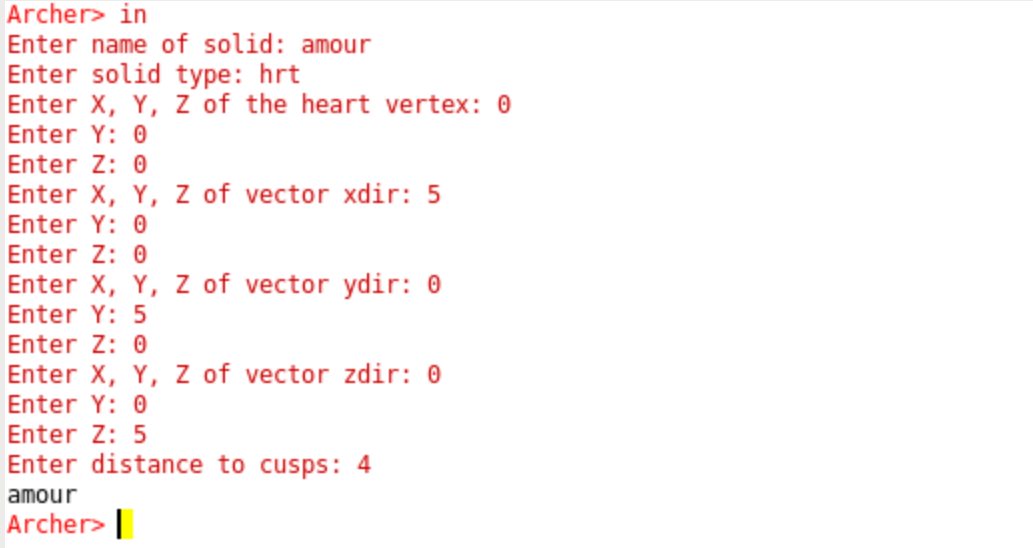
\includegraphics[trim=0.0cm 0.5cm 0.1cm 0.1cm, clip=true, totalheight=0.4\textheight]{Pictures/Typein.png}
\caption[Testing type in support for the heart-­shaped primitive in archer]{Testing type in support for the heart­-shaped primitive in archer}
\label{Typein}
\end{figure}

\clearpage

%----------------------------------------------------------------------------------------------------------------

%----------------------------------------------------------------------------------------------------------------
%						SECTION 2
%----------------------------------------------------------------------------------------------------------------
\section{Formatted description of the heart­-shaped primitive}

After   having   created   objects   for   modeling,   it   sometimes   becomes  
necessary   to   display   a   description   of   these   objects.   For   us   to   test   that   we   can  
describe   the   heart­shaped   primitive,   we   used   BRL-­CAD's   \textit{\textbf{l}}[39]   command   on  
the   amour   object.   The   \textit{\textbf{l (listing)}}   command   displays   a   verbose   description   of   a
 specific   list   of   objects.   If   the   shape   of   the   object   is   a   primitive,   then   detailed  
parameters   of   that   shape   are   displayed.   If   the   object   is   a   combination   of   other  
primitives,   then   the   boolean   formula   for   the   combination   is   listed   while   indicating  
any   accumulated   transformations.   If   a   shader   and   colour   has   been   assigned   to  
the   combination,   then   all   details   will   be   listed.   The   \textit{\textbf{-­t}}   (terse)   option   displays   a  
shorter list of primitive shape parameters.

\hspace{30} To   describe   the   \textit{amour}   object,   we   print   amour's   parameters   in   both   terse  
and   verbose   forms   by   running   the   \textit{\textbf{“l -t amour”}}   and   \textit{\textbf{“l amour”}}   commands  
respectively in the archer command prompt. This is shown in Figure 4.2 below.

\begin{figure}[htbp]
\centering
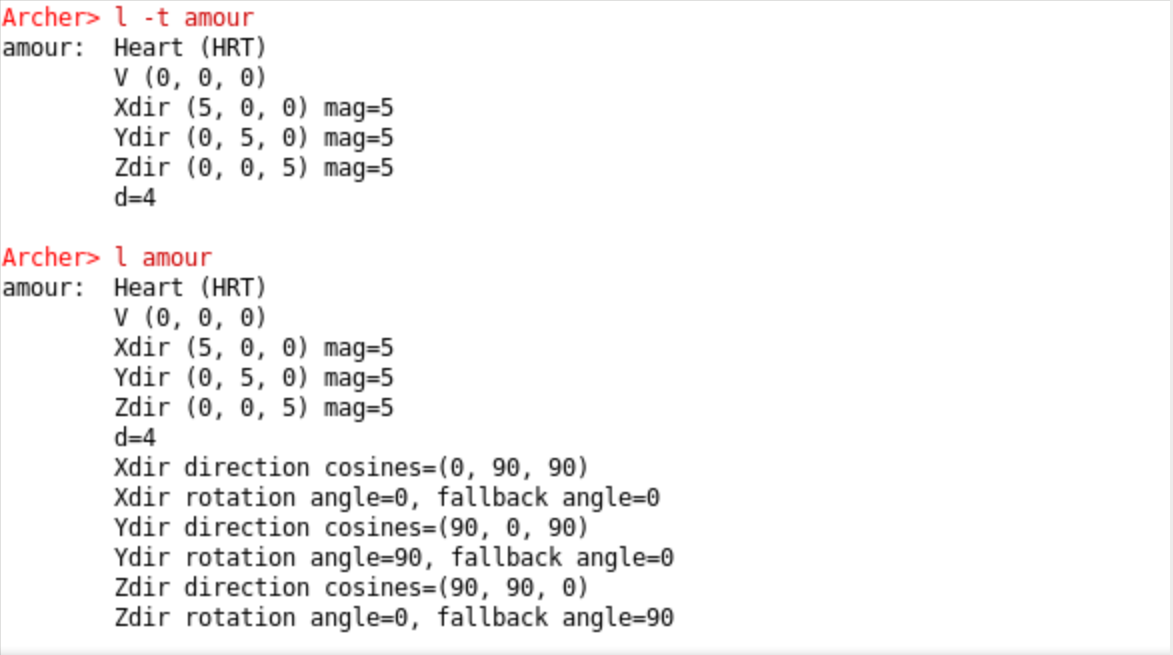
\includegraphics[trim=0.0cm 0.5cm 0.1cm 0.1cm, clip=true, totalheight=0.4\textheight]{Pictures/Describe.png}
\caption[Testing the formatted description of the heart­-shaped primitive]{Testing the formatted description of the heart­-shaped primitive}
\label{Describe}
\end{figure}

\clearpage

%-------------------------------------------------------------------------------------------------------------------------------

%-------------------------------------------------------------------------------------------------------------------------------
%					SECTION 3
%-------------------------------------------------------------------------------------------------------------------------------

\section{The bounding box of the heart-­shaped primitive}

As   we   earlier   stated,   the   $rt\_hrt\_bbox()$   function   was   implemented   to
 calculate   the   bounding   box   of   the   heart-­shaped   primitive.   In   order   to   test   that  
the   bounding   box   of   the   heart-­shaped   primitive   is   computed,   we   use  
BRL­-CAD's \textit{\textbf{bb}}[40] command.

\hspace{30} The   \textit{\textbf{bb (bounding box)}}  command   reports   dimensional   information   about   objects   using  
bounding   boxes.   It   does   this   by   calculating   an   axis­aligned   bounding   box   for   an  
object   and   printing   the   dimensions   of   that   box   to   the   command   prompt   of  
archer.   The   \textit{\textbf{bb}}   command   support   various   options,   most   of   which   control   the  
type of information reported.  

\begin{itemize}
\item The \textit{\textbf{-­e} (extent)} option reports the extent of the bounding box by printing its minimal and maximal points.  
\item The \textit{\textbf{-­d} (default)} option reports the length, width and height of the box.  
\item The \textit{\textbf{-­v} (volume)} option prints the volume of the bounding box by default too.  
\item The \textit{\textbf{-­q} (quiet)} option prints the properties of an object in quiet mode by disabling the printing of the default header.
\end{itemize}

\hspace{30} Once   more   we   use   the   amour   object   and   the   \textit{bb}   command   to   test   how  
effectively   the   bounding   box   of   the   heart­-shaped   primitive   was   implemented.  
To   report   the   extent   of   the   bounding   box   of   the   amour   object,   we   print   its  
minimal   and   maximal   points   by   running   the   \textit{\textbf{“bb   ­-qe   amour”}}   command   in   either  
the   mged   or   archer   command   prompts.   Then,   we   ran   the   \textit{\textbf{“bb   -­qv   amour”}}  
command   in   archer   so   that   the   volume   of   the   amour   object   is   reported   in   cubic  
millimeters.   After,   we   reported   the   length,   width   and   height   of   amour's   bounding  
box   by   running   the   \textit{\textbf{“bb   ­-qd   amour”}}.   Finally,   to   report   the   volume   and  
dimensions   of   the   bounding   box,   we   ran   the   \textit{\textbf{“bb   amour”}}   command   in   archer's  
command prompt. 

\hspace{30} The image above in Figure 4.3 shows the results obtained after running the aforementioned commands. 

\begin{figure}[htbp]
\centering
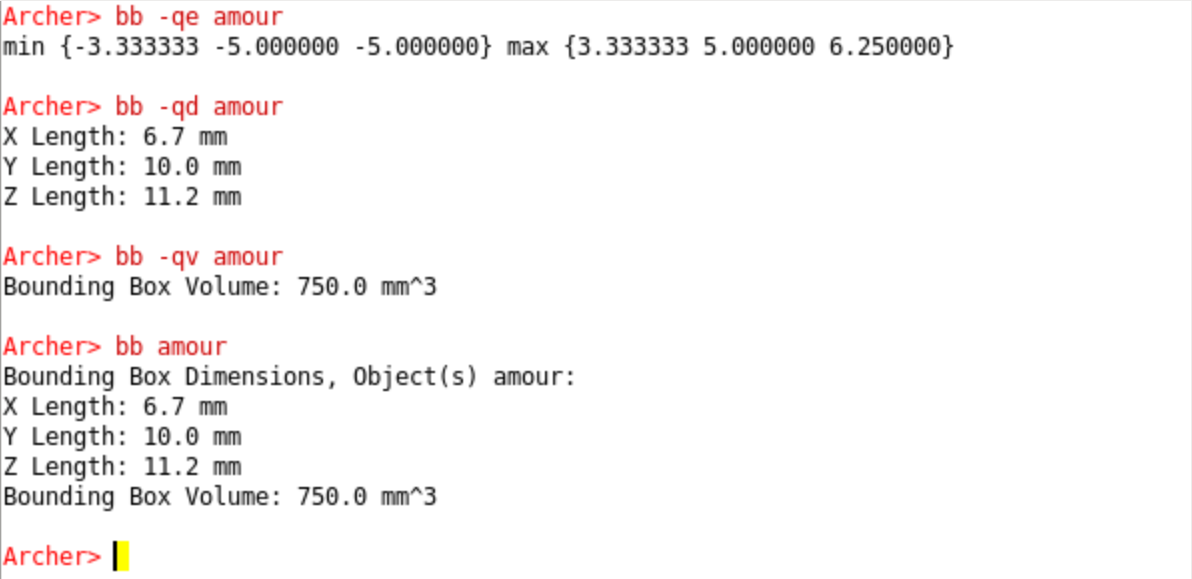
\includegraphics[trim=0.0cm 0.5cm 0.1cm 0.1cm, clip=true, totalheight=0.4\textheight]{Pictures/Bounding.png}
\caption[Testing the bounding box of the heart­-shape]{Testing the bounding box of the heart­-shape}
\label{Bounding}
\end{figure}

\clearpage

%---------------------------------------------------------------------------------------------------------------------

%---------------------------------------------------------------------------------------------------------------------
%				SECTION 4
%---------------------------------------------------------------------------------------------------------------------
\section{Plotting the wireframe of the heart­-shaped primitive}

\hspace{30} The   process   of   modeling   sometimes   warrants   the   preview   of   the   skeleton  
of   a   specific   set   of   objects.   To   test   that   the   wireframe   of   the   heart­-shaped  
primitive   is   working,   we   use   the   \textit{\textbf{draw}}[41]   command   in   BRL­-CAD.   The   \textit{\textbf{draw}}  
command   displays   objects   in   either   the   mged   or   archer   interfaces.   It   is  
synonymous   to   BRL­-CAD's   \textit{\textbf{e}}   command.   The   draw   command's   \textit{\textbf{-­C} (colour)}  
option   enables   the   user   to   specify   a   colour   that   overrides   all   other   previous  
colour specifications.  

\hspace{30} To   draw   the   wireframe   of   the   amour   object   using   white   wires,   we   run   the  
\textit{\textbf{“draw -­C 255/255/255 amour”}}   command.   The   image   in   Figure   4.4   below   shows  
the wireframe of amour with red iso­contours.  

\begin{figure}[htbp]
\centering
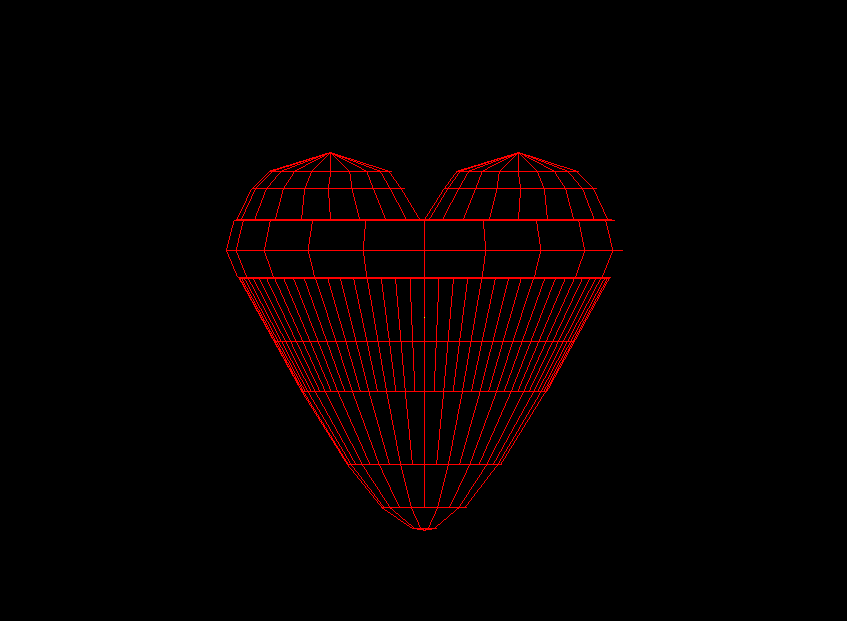
\includegraphics[trim=0.0cm 0.5cm 0.1cm 0.1cm, clip=true, totalheight=0.4\textheight]{Pictures/Wireframe.png}
\caption[Testing the wireframe of the heart­shaped primitive]{Testing the wireframe of the heart­shaped primitive}
\label{Wireframe}
\end{figure}

%---------------------------------------------------------------------------------------------------------------------

%---------------------------------------------------------------------------------------------------------------------
%				SECTION 5
%---------------------------------------------------------------------------------------------------------------------

\section{Ray tracing and surface representation of the heart-­shaped primitive}

\hspace{30} Ray­tracing   the   heart­-shaped   primitive   is   the   most   important   geometric  
property   because   the   others   lose their relevance without   BRL­-CAD's   capacity   to   render  
the   heart­-shaped   primitive.   A   major   difficulty   during   the   raytracing   of   the  
heart­-shaped   primitive   was   the   misunderstanding   that   the   sextic   equation   could  
be solved in radicals and only algebraic methods can be employed to solve it.  

\hspace{30} In   order   to   test   that   the   ray­tracing   property   of   the   heart­-shaped   primitive  
works, we use BRL-­CAD's \textit{\textbf{rt}}[42] command. The \textit{\textbf{rt}} command ray­traces a set
 of objects with the default option of \textit{\textbf{-­s50}}. Like other BRL­-CAD commands, it has various options.

\begin{itemize}
\item The \textit{\textbf{-a} (azimuth)} option enables the designer to specify the azimuth at which the rendered image will be created.  
\item The \textit{\textbf{-­e} (elevation)} option enables the designer to specify the elevation at which the rendered image should be created.  
\item The \textit{\textbf{-w} (width)} option enables the designer to specify the width of the rendered image.  
\item The \textit{\textbf{-­n} (height)} option enables the designer to specify the height of the rendered image.  
\item The \textit{\textbf{-­s} (size)} option enables the designer to specify the length of the rendered image (which is a square).  
\item The \textit{\textbf{-­C} (colour)} option enables the designer to specify the colour of the rendered image's background.  
\item The \textit{\textbf{-­o} (output)} option enables the designer to specify the name of the rendered image.
\end{itemize}

\clearpage
%----------------------------------------------------------------------------------------------------------------------

\hspace{30} Using the \textit{\textbf{rt}} command in BRL-­CAD, we produced 360 images each at an  
azimuth angle of 1 degree from the other and an elevation angle of 35 degrees from our viewpoint.
The width and height   of   these   images   were   640   and   480  
pixels   respectively. To   do   this,   we   edited   the   Fly­Around   Animation   script   [43]  
on BRL­-CAD's website which is shown below;

\begin{verbatim}
        #!/bin/sh 
        for i in `loop 000 359 1`; do 
            rt -­a $i ­-e 35 -­w 640 -­n 480 -­o image$i.png heart_example.g amour 
        done \end{verbatim}

Figure 4.5 below shows some images of the heart­-shaped primitive obtained from running the script above.

\begin{figure}[htbp]
\centering

\includegraphics[trim=0.0cm 0.5cm 0.1cm 0.1cm, clip=true, totalheight=0.4\textheight]{Pictures/Besides.png}
\begin{minipage}{0.2\textheight}
\begin{flushleft}

\includegraphics[width=4cm,height=2cm, clip=true, totalheight=0.17\textheight]{Pictures/Above.png}
\end{flushleft}
\end{minipage}
\begin{minipage}{0.2\textheight}
\begin{flushleft}

\includegraphics[width=4cm,height=2cm, clip=true, totalheight=0.17\textheight]{Pictures/Below.png}
\end{flushleft}
\end{minipage}
\caption[Images rendered after ray­tracing the heart­-shaped primitive]{Images rendered after ray­tracing the heart-­shaped primitive}
\label{Besides}
\end{figure}

The   first   image   shows   the   heart-­shaped   primitive   upfront   with   its   two   lobes   and  
2   cusps   just   as   its   data   structure   was   designed.   The   other   two   images   show  
that   the   heart­-shaped   primitive   is   elliptical   on   the   XY   and   XZ   planes   as   we  
earlier highlighted when testing its wireframe.

\hspace{30} After   appropriately   sequencing   these   images   with   padded   zeroes,   we  
used   the   ImageMagick   \textit{convert}   command   to   composite   them   into   a   single  
animated   image.   Several   animations   were   produced   showing   the   heart­shaped  
primitive   spinning   from   several   viewpoints   (above, below and besides )   and  
these   can   be   viewed   on   my   youtube   channel [44] .These   animations   are   proof   that  
artists   can   indeed   use   the   BRL-­CAD   software   to   produce   cartoon   animations,  
design   cards,royal   seals   and   banners,   gifts,   magnificient   embroidery   and  
presents   for   family   and   communal   celebrations   such   as   weddings,   family  
reunions and Valentine's day for entertainment and fashion.
\clearpage
%-------------------------------------------------------------------------------------------------------------------------
 
%-----------------------------------------------------------------------------------------------------------------
\chapter{CONCLUSIONS}
\label{Conclusions}
\lhead{Chapter 5. \emph{Conclusions}} 
%-----------------------------------------------------------------------------------------------------------------

\hspace{30} In   this   chapter,   we   note   the   new   and   original   contributions   of   our   work   on  
the   heart-­shaped   primitive   to   the   field   of   CAD   and   highlight  
possible   research   orientations   which   can   spring   up   from   it.   During   our   work,   we  
first   designed   the   heart­-shaped   primitive's   structure,   wrote   necessary   callback  
functions and tested them using BRL-­CAD's inbuilt testing infrastructure. 

%----------------------------------------------------------------------------------------
%	SECTION 1
%----------------------------------------------------------------------------------------

\section{Our Contribution}

The contributions of this thesis are outlined below;  

\begin{itemize}
\item We   showed   that   BRL-­CAD's   Laguerre-­based   root   solver   is   indeed   a  
sure­fire   iterative   method   for   finding   roots   of   polynomials   and   ascertained  
it's stability on sextic equations.  
\item This   work   provides   a   guideline   for   the   development   of   primitives   within  
open   source   CAD   software   by   highlighting   the  implementation   of   
geometrically­ useful properties for the heart-shaped primitive within BRL-­CAD.  
\item By   producing   animated   videos   from   resulting   rendered   images,   we  
showed   that   BRL­-CAD   is   a   software   package   which   artists   can   use   to  
produce   cartoon   animations,   design   cards,royal   seals   and   banners,   gifts  
and   presents   for   family   and   communal   celebrations   such   as   weddings,  
valentine's day, etc, for entertainment purposes.
\end{itemize}

%--------------------------------------------------------------------------------------------------
%		SECTION 2
%--------------------------------------------------------------------------------------------------

\section{Further Research}

\hspace{30} In   order   to   invite   more   artists   to   use   BRL-­CAD   for   the   creation   of  
entertainment   content   and   enhance   BRL-­CAD's   functionality   so   that   it   becomes  a 
better   open   source   CAD   package,   we   propose  the following research ideas;

\begin{itemize}
\item Although   the   heart-­shaped   primitive   has   been   shown   to   have   possess   a  
wireframe   and   an   implicit   surface   representation,   it   would   be   nice   for   this  
primitive   to   own   an   explicit   surface   representation   based   on   its   parametric  
equations.  
\item BRL­-CAD   is   used   within   the   scientific   community   for   research   and  
computer   graphics   education,   it   would   be   nice   to   investigate   the   stability  
of   BRL-­CAD's   Laguerre­-based   root   solver   on   septic,   octic   and   nonic  
equations which are monic polynomials of order 7, 8 ans 9 respectively.  
\item Since   BRL-­CAD   boasts   of   more   than   400   commands   within   its   pocket,   it  
would   be   worthwhile   to   invite   more   artists   within   the   entertainment   industry  
by   adding   more   functionality   to   its   animate   command   so   that   several  
images can be combined into animated videos.
\end{itemize}

\clearpage

%--------------------------------------------------------------------------------------------------------
 

\clearpage % Start a new page

%----------------------------------------------------------------------------------------
%	BIBLIOGRAPHY/REFERENCES
%----------------------------------------------------------------------------------------
\newgeometry{a4paper,lmargin=2.6in,rmargin=0.2in,tmargin=2.5in,bmargin=0in}
\begin{center}
\Large\textbf{REFERENCES}\\
\end{center}

[1] Wikipedia, “Drawing — Wikipedia, the free encyclopedia,” 2014. [Online] Available:
https://en.wikipedia.org/wiki/Drawing. [Accessed: March. 17].

[2] K. J. Weiler, Topological structures for geometric modeling. PhD thesis, Rensselaer
Polytechnic Institute, Troy, New York, 1986.

[3] C. S. Morrison, Harmanpreet S., Nyah C., Isaac K., Yapp C., & Scott N., \textit{Hacking
 BRL-CAD A Contributor’s guide}. Weesperstraat 3 1018 DN Amsterdam The
Netherlands: FLOSS Manuals Foundation, 1 ed., 10 2013. Google Documentation Camp.

[4] Requicha A. A. & Tilove R.B.,, “Mathematical models of rigid solid objects,” Tech.
Rep. 28, University of Rochester, Production Automation Project, Rochester, New York, 11 1977.

[5] A. A. Requicha, “Representations for rigid solids: Theory, methods and systems,”
ACM Computing Surveys, vol. 12, p. 437 – 464, 12 1980.

[6] Markowsky G., & Wesley M.A., “Fleshing out wireframes,” IBM Journal of Research
and Development, vol. 24, pp. 229 – 258, 9 1980.

[7] Sederberg T.W., \textit{Implicit and Parametric Curves and Surfaces for Computer Aided
Geometric Design}. PhD thesis, Purdue University, Lafayette, Indiana, 1983.

[8] Buchberger B., “Grobner bases, gaussian elimination and resolution of systems of
algebraic equations,” Multidimensional Systems Theory, vol. 24, p. 184 – 232, 9 1980.

[9] Lazard D., “Grobner bases, gaussian elimination and resolution of systems of algebraic
equations,” EUROCAL ’83, Lectures Notes in Computer Science, vol. 2, p. 146 – 156, 10 1983.

[10] Hoffmann C. M., \textit{An Introduction To Geometric and Solid Modeling}. San Francisco,
California: Morgan Kaufmann Publishers, 1 ed., 1989.

[11] Faugere. J., Gianni. P., Lazard. D., & Mora. T, “Efficient change of ordering for
grobner bases of zero-dimensional ideals.” manuscript.

[12] S. Abhyankar & C. Bajaj, “Automatic rational parameterization of curves and sur-
faces ii: Conics and conicoids,” Computer-Aided Design, vol. 19, pp. 11–14, 7 1987.

[13] G. Golub & C. Van Loan, \textit{Matrix Computations}. John Hopkins University Press, 1 ed., 1977.

[14] Weiler K., “Edge-based data structures for solid modeling in curved-surface environments,”
 IEEE Computer Graphics and Applications, vol. 21, 1 1985.

[15] Woo T. C., “A combinatorial analysis of boundary structure schemata,” IEEE Computer 
Graphics and Applications, vol. 19, 3 1985.

[16] Baumgart B.,, “Winged-edge polyhedron representation,” Tech. Rep. 320, Stanford 
University, Palo Alto, California, 1972.

[17] I. C. Braid, R. C. Hillyard, & I. A. Stroud, \textit{Stepwise Construction of polyhedra in
geometric modeling}. New York: Academic Press, 1 ed., 1980.

[18] F. Yamaguchi & T. Tokieda, “Bridge edge and triangulation approach in solid modeling,” 
Frontiers in Computer Graphics 84, ́pp. 44–65, 1985. Springer-verlag.

[19] M. Mantyla, \textit{An introduction to SOLID MODELING}. Computer Science Press, 1 ed.,1988.

[20] P. M. Hanrahan, Topological Shape Models. PhD thesis, University of Wisconsin,
Madison, Wisconsin, 1985.

[21] S. Ansaldi,L. De Floriani, & B. Falcidieno, “Geometric modeling of solid objects by
using a face adjacency graph representation,” Proceedings ACM Siggraph ’85, pp. 131 – 139, 1985.

[22] V. Shapiro & D. Vossler., “BREP to CSG conversion I: Representations,” Tech.Rep. 89,
 Mechanical and Aerospace Engineering, Cornell University, Ithaca, New York, 1990.

[23] A. A. Requicha & H. B. Voelcker, “Constructive solid geometry,” Tech. Rep. 25,
Production Automation Project, University of Rochester, Rochester, New York, 11 1977.

[24] A. Klinger & C.R.Dyer., “Experiments in picture representation using regular decomposition,”
 Computer Graphics and Image Processing, vol. 5, pp. 68 – 105, 3 1976.

[25] G. M. Hunter, \textit{Efficient computation and data structures for computer graphics}. PhD thesis, 
Department of Electrical and Computer Science, Princeton University, Princeton, New Jersey, 1978.

[26] R. A. Finkel & J. L. Bentley, “Quadtree: A data structure for retrieval on composite keys,”
 Acta Informatica, vol. 4, no. 1, pp. 1–9, 1974.

[27] E. Kawaguchi & T. Endo, “On a method of binary picture representation and its application to
 data compression,” IEEE Transaction in Pattern Analysis and Machine Intelligence, vol. 2, p. 27 – 35, 1 1980.

[28] K. Hinrichs & J. Nievergelt., “The grid file : a data structure designed to support
proximity queries on spatial objects,” International Workshop on Graph Theoretic Concepts
 in Computer Science, pp. 100 – 113, 1983. Trauner Verlag, Linz, Austria.

[29] A. Guttman, “R-trees: a dynamic index structure for spatial searching,” Proceedings
of the SIGMOD Conference, pp. 47 – 57, 1984. Boston, New York.

[30] H. Samet & R. E. Webber., “Storing a collection of polygons using quadtrees,” ACM
Transactions on Graphics, vol. 4, p. 182 – 222, 7 1985.

[31] M. Karasick, \textit{On the Representation and Manipulation of rigid Solids}. PhD thesis,
McGill University, Montreal, Canada, 1988.

[32] G. Vanecek Jr., \textit{Set Operations on Polyhedra using Decomposition methods}. PhD
thesis, University of Maryland, College Park, Maryland, 1989.

[33] Eric S. Raymonds, “How to become a hacker.” Available : 

http://www.catb.org/esr/faqs/hacker-howto.html. [Accessed :June 30, 2014].

[34] Sourceforge, “Find, create, and publish open source software for free.” 
[Online].Available: http://sourceforge.net. [Accessed :July 15, 2014].

[35] GitHub, “Build software better, together.” [Online]. Available: 

https://github.com. [Accessed :July 15, 2014].

[36] BRL-CAD User Commands.,“MGED commands.”[Online].Available:

http://www.brlcad.org/wiki/MGED Commands.[Accessed :July 15, 2014].

[37] BRL-CAD in user command, “IN.” [Online].Available : http://manned.org/in.n. 
[Accessed :July 16, 2014].

[38] BRL-CAD l user command, “L.” [Online].Available : http://manned.org/l.n. 
[Accessed :July 16, 2014].

[39] BRL-CAD bb user command, “BB.” [Online].Available : http://manned.org/bb.n. 
[Accessed :July 16, 2014].

[40] BRL-CAD draw user command, “DRAW.” [Online]. Available:

http://manned.org/draw.n. [Accessed :July 16, 2014].

[41] BRL-CAD rt user command, “RT.” [Online].Available : http://manned.org/rt.n. 
[Accessed :July 16, 2014].

[42] BRL-CAD Animation page, “Animation.” [Online]. Available:

http://brlcad.org/wiki/Animation.[Accessed :July 16, 2014].

[43] Isaac K., “BRL-CAD heart-shaped primitive viewed from its bottom.” [Online].
Available : https://www.youtube.com/watch?v=DxrJ2vIrHCUfeature=youtu.be.
[Accessed :July 16, 2014].

[44] Isaac K., “BRL-CAD symbol of love.”[Online].

Available: https://www.youtube.com/watch?v=ErmljjeY-A.[Accessed :July 16, 2014].

%\label{References}

%\lhead{\emph{References}} % Name the Page header "References"

%\bibliographystyle{ieeetr} % Use the "ieeetr" BibTeX style for formatting the References

%\bibliography{References} % The references information are stored in the file named "References.bib"


%----------------------------------------------------------------------------------------
%	THESIS CONTENT - APPENDIX
%----------------------------------------------------------------------------------------
\newgeometry{a4paper,lmargin=2.6in,rmargin=0in,tmargin=1.3in,bmargin=0in}

\backmatter

\appendix % Tell LaTeX that the following 'chapters' are Appendices

\lhead{\emph{Appendix}}

\chapter{APPENDIX} % Main appendix title

\label{Appendix} % For referencing this appendix elsewhere, use \ref{AppendixA}

\lhead{Appendix . \emph{Appendix}} % This is for the header on each page - perhaps a shortened title

Coefficients of the terms in equation \textit{(7)} \\

$C_6  = 4320a^2b^2c^2 + 960a^2c^2(a^2 + c^2) + 320(a^6 + c^6) + 2160b^2(a^4 + c^4) + 4860b^4(a^2 
+ c^2) - 36b^3c^3 + 3645b^6$
  
$C_5  = 8640(ax_0b^2(a^2 + c^2) + by_0a^2c^2  + cz_0b^2(a^2 + c^2)) + 9720b^4(ax_0 + cz_0) + 1920(a^4 
+ c^4(ax_0 + cz_0)) + 4320(a^4 + c^4by_0) + 3840(a^2 + c^2)(ax_0 + cz_0) + 19440(c^2b^2 + ab^2) 
by_0 -­ 108bc(c^2by_0 + cz_0b^2) -­ 320a^2ba^3 + 21870y_0b^5$  

$C_4  = 4320(a^2(b^2z_0^2 + c^2y_0^2) + b^2(x_0^2c^2 - a^2 - c^2)) -­ 960(a^4(1 -­ z_0^2) + c^4 + b^2(a^2y_0 ­- 
b^2x_0^2)) + 4860(b^4(x_0^2 + z_0^2 -­ 1)) + 4800(a^4x_0^2 + c^4z_0^2)+ 2160y_0^2(a^4 + c^4) + 
5760a^2c^2(x_0^2 + z_0^2) + 7680ax_0cz_0(a^2 + c^2) + 17280((ax_0by_0 + by_0cz_0 )(a^2 + c^2) + 
ax_0cz_0b^2) + 12960b^2(a^4x_0^2 + c^4z_0^2) + 29160b^2y_0^2(a^2 + c^2) -­ 108bc(b^2z_0^2 + c^2y_0^2)
- 1920a^2c^2 -­ 54675y_0^2b^4 -­ 324z_0c^2b^2y_0 - 640ax_0b^3$    

$C_3 = 3840(ax_0 + cz_0)(a^2z_0^2 + c^2x_0^2 - a^2 + c^2) + 8640(ax_0(z_0^2b^2 + c^2y_0^2 + b^2x_0^2 + 
a^2y_0^2 -­ b^2) + by_0(a^2z_0^2 + c^2x_0^2 - a^2 - c^2) + cz_0(a^2y_0^2 + b^2x_0^2 + bz_0^2 + c^2y_0^2 - ­ b^2)) + 6400 
(a^3x_0^3 + c^3z_0^3) + 19440by_0(b^2(x_0^2 + z_0^2 -­ 1) + y_0^2(a^2 + c^2)) -­ 36(b^3z_0^3 + c^3y_0^3 ) + 
11520(ax_0cz_0(ax_0 + cz_0))­ - 324by_0cz_0(bz_0 + c + y_0) + 25920by_0(z_0^2c^2 + x_0^2a^2) ­- 
320x_0^2b^3  + 72900y_0^3b^3 + 34560ax_0by_0cz_0 + 58320ax_0b^2y_0^2 -­ 1920ax_0b^2y_0 + 
58320cz_0b^2y_0  -­ 960a^2by_0^2$

$C_2 = 960(a^2(1 + z_0^4) +  c^2(1 + x_0^4) - b^2x_0^2y_0) + 2160b^2(1 + x_0^4 + z_0^4) + 4320(y_0^2( 
a^2 + c^2 + a^2z_0^2 + c^2x_0^2) + b^2(x_0^2z_0^2 - x_0^2­ - z_0^2)) + 4800(x_0^3a^2 + z_0^3c^2)
 + 4860y_0^4(a^2 + c^2) + 5760(z_0^2c^2(1 + x_0^2) + x_0^2a^2(z_0^2 - ­1)) + 7680ax_0cz_0(x_0^2 + z_0^2 - 1­ - 1920(a^2z_0^2 + c^2x_0^2 + ax_0y_0^2b) + 17280(by_0(ax_0^3 - ax_0 + cz_0^3 -­ cz_0 + az_0^2) + ax_0cz_0y_0^2) + 38880bz_0^3(ax_0 + cz_0) + 12960y_0^2(a^2x_0^2 ­- c^2z_0^2) + 
29160b^2y_0^2(x_0^2 + z_0^2 -­ 1) ­- 180y_0z_0c^2y_0^2 + b^2z_0^2) ­- 320a^2y_0^3 + 54675y_0^3b^2$  

$C_1  = 1920((ax_0 + cz_0)(1 + x_0^4 + z_0^4)) + 4320by_0(1 + x_0^4 + z_0^4) + 8640(-­by_0z_0^2 + 
ax_0z_0^2y_0^2 + cz_0x_0^2y_0^2 + by_0^2x_0z_0^2 -­ ax_0y_0^2 + ay_0^2 + ax_0^3y_0^2 -­ cz_0y_0^2 + cz_0^3y_0^2 - by_0x_0^2) -­ 
3840(cz_0^3 + ax_0^3 + ax_0z_0^2 - ­ax_0^2z_0^2 + cz_0x_0^2 -­ cz_0^3x_0^2) -­ 19440(by_0^3(1 -­ x_0^2 -­ z_0^2)) + 
9720(y_0^4(ax_0 + cz_0)) + 21870(by_0^4)­ - 640(ax_0y_0^3 - by_0^2x_0^2) -­ 108(cz_0^2y_0^2 + by_0^2y_0^3)$
 
$C_0 = 320(-­x_0^6 + z_0^6 - x_0^2y_0^3) + 960(x_0^2 + z_0^4x_0^4 + x_0^2z_0^4 -­ x_0^4 -­ z_0^4) + 4320(x_0^2y_0^2z_0^2 -­ 
x_0^2y_0^2 -­ z_0^2y_0^2) ­- 1920x_0^2z_0^2 - ­36x_0^3y_0^3 + 2160(y_0^2(1 + x_0^4 + z_0^4)) + 4860(y_0^4(x_0^2 + z_0^2  
+ 1)) + 3645y_0^5$


\end{document}  
